% Isaac Dunn Part II Computer Science Dissertation
\documentclass[12pt,a4paper,twoside,openright]{report}
\usepackage[pdfborder={0 0 0}]{hyperref}    % turns references into hyperlinks
\usepackage[margin=25mm]{geometry}  % adjusts page layout
\usepackage[T1]{fontenc}
\usepackage{mathpazo}  % style
\usepackage{graphicx}  % allows inclusion of PDF, PNG and JPG images
\graphicspath{ {./figs/} }
\DeclareGraphicsExtensions{.pdf,.png,.jpg}
\usepackage{verbatim}
\usepackage{docmute}   % only needed to allow inclusion of proposal.tex
\usepackage{amsmath}
\usepackage{amsfonts}
\usepackage{algorithm}
\usepackage[noend]{algpseudocode}
\usepackage{enumitem}
\usepackage{color}
\usepackage{listings}
\usepackage{subcaption}
\usepackage[labelfont=bf]{caption}
\usepackage[sort,nocompress]{cite} % sort multiple citations, but don't group

\definecolor{dkgreen}{rgb}{0,0.6,0}
\definecolor{grey}{rgb}{0.5,0.5,0.5}
\definecolor{mauve}{rgb}{0.58,0,0.82}
\lstset{ % style of code listings
	frame=tb,
	language=ML,
	aboveskip=3mm,
	belowskip=3mm,
	showstringspaces=false,
	columns=flexible,
	basicstyle={\small\ttfamily},
	numbers=none,
	numberstyle=\tiny\color{grey},
	keywordstyle=\color{blue},
	commentstyle=\color{dkgreen},
	stringstyle=\color{mauve},
	breaklines=true,
	breakatwhitespace=true,
	tabsize=4
	}


\raggedbottom                           % try to avoid widows and orphans
\sloppy
\clubpenalty1000%
\widowpenalty1000%

\renewcommand{\baselinestretch}{1.1}    % adjust line spacing to make
                                        % more readable

% "let a = b in" for use in algorithms
\newcommand{\Let}[2]{\State \textbf{let} #1 = #2 \textbf{in}}

% For use in the happens-before relation varient
\newcommand{\longhookrightarrow}
	{\ensuremath{\lhook\joinrel\longrightarrow}}


\newenvironment{understandinglist}
	{\begin{itemize} \itemsep 0em}{\end{itemize}}

\newenvironment{figtile} % for evaluation graphs
{\begin{subfigure}{0.48\textwidth}
		\def\svgwidth{\textwidth}
		\captionsetup{font=footnotesize}
	}
	{\end{subfigure}}

\begin{document}

\bibliographystyle{plain}


%%%%%%%%%%%%%%%%%%%%%%%%%%%%%%%%%%%%%%%%%%%%%%%%%%%%%%%%%%%%%%%%%%%%%%%%
% Title page


\pagestyle{empty}

\rightline{\LARGE \textbf{Isaac Dunn}}

\vspace*{60mm}
\begin{center}
\Huge
\textbf{Dynamic Partial-Order Reduction for Model Checking} \\[7mm]
Computer Science Tripos -- Part II \\[6mm]
Clare College \\[7mm]
\LARGE \today  % today's date
\end{center}

%%%%%%%%%%%%%%%%%%%%%%%%%%%%%%%%%%%%%%%%%%%%%%%%%%%%%%%%%%%%%%%%%%%%%%%%%%%%%%
% Proforma, table of contents and list of figures

\pagestyle{plain}

\chapter*{Proforma}

{\large
\begin{tabular}{ll}
Name:           & \bf Isaac Dunn                            			 \\
College:        & \bf Clare College                    				     \\
Project Title:	& \bf Dynamic Partial-Order Reduction for Model Checking \\
Examination:    & \bf Computer Science Tripos -- Part II, June 2016      \\
Word Count:     & \bf N    												 \\
Project Originator: & \bf Isaac Dunn\footnotemark[1] 					 \\
Supervisors:	& \bf Dr. Jonathan Hayman \& Prof. Glynn Winskel         \\
\end{tabular}
}
\footnotetext[1]{with guidance from Dr. Jonathan Hayman}
\stepcounter{footnote}


\section*{Original Aim of the Project}

The original aim of the project was to implement
a simple model-checking algorithm, and to
understand and implement the dynamic partial-order reduction
model-checking algorithm.

\section*{Work Completed}

The original dynamic partial-order reduction algorithm
was successfully implemented, with several extensions
also completed, including implementation of a stateful
model-checking algorithm, a stateful adaptation of the
dynamic partial-order reduction algorithm, application
of the sleep-set technique to both a simple model checker
and the dynamic partial-order reduction algorithm,
and the implementation of a static partial-order reduction
algorithm. A quantitative comparison of the implemented
algorithms was also completed.

\section*{Special Difficulties}

No special difficulties were encountered.
 
\section*{Declaration of Originality}

I, Isaac Dunn of Clare College, being a candidate for Part II of the Computer
Science Tripos, hereby declare
that this dissertation and the work described in it are my own work,
unaided except as may be specified below, and that the dissertation
does not contain material that has already been used to any substantial
extent for a comparable purpose.

\bigskip
\leftline{Signed:}

\bigskip
\leftline{Date:}

\setcounter{tocdepth}{1} % hide subsections
\tableofcontents

%\newpage
%\section*{Acknowledgements}
%
%Put acknowledgements here.

%%%%%%%%%%%%%%%%%%%%%%%%%%%%%%%%%%%%%%%%%%%%%%%%%%%%%%%%%%%%%%%%%%%%%%%
% now for the body

\pagestyle{headings}

\chapter{Introduction}
After reading this chapter,
you should understand:
\begin{understandinglist}
	\item what model checking is and why it is useful;
	\item what the state explosion problem is;
	\item how partial-order reduction
	techniques address the state explosion problem;
	\item the aims of my project; and
	\item the aims of this dissertation.
\end{understandinglist}

\section{Model Checking}
%After reading this section,
%you should understand why formal methods for
%verifying the correctness of software and
%hardware systems are useful, that model
%checking is such a formal method, and
%how model checking works.

There are many reasons for ensuring that
software and hardware systems have as
few defects as possible. Failure of a
safety- or mission-critical system can
have devastating consequences, but even the
presence of bugs in everyday commercial systems has
serious economic consequences; in 2002,
software bugs were estimated to cost
the U.S. economy \$59.5 billion per year \cite{tass02}.

Complimentary to traditional testing methods
and peer review, formal verification methods have been
increasing in popularity as a strategy
to minimise the number of defects in a
software or hardware system. A formal
method uses some form of automated
mathematical analysis to increase
the confidence that a system meets its
specification, or shows that it does not.

Model checking is a category of formal
verification techniques
that explore all possible system states in a
brute-force manner \cite{bai08}. In particular,
given a formal model of a system, and a
formal specification of a property, a model
checking algorithm automatically checks whether the
system satisfies that property by an
exhaustive search of the state space.
Model checking has been used with considerable
success in practice, for instance in verifying
software controlling a flood barrier near
Rotterdam \cite{kars96},
a NASA Mars Rover \cite{brat04},
and an ``industrial-size design of an
ultra-modern satellite platform'' \cite{est12}.

\section{The State Explosion Problem}
%After reading this section, you should
%understand what the state explosion problem
%is, and its implications for model checking.

One of the advantages of model checking is
that it can be used to verify that concurrent
systems are free of deadlocks, livelocks, or
obscure race conditions that could result in
an error, whereas such exposing such defects
using solely conventional testing is notoriously
difficult, since when the operating system
schedules the different processes to run
cannot be specified or known in advance by the
test engineer. However, model checking does
suffer from what is known as the
\textit{state explosion problem} when verifying
concurrent systems.

Consider a concurrent system consisting
of $n$ different processes, each of which
has $k$ instructions to execute before it
terminates. Suppose that the threads are
executed asynchronously, so that the next
process to run is always decided non-deterministically
from all possibilities.
How many possible different executions are there?
That is, how many different interleavings of
the instructions of the different threads are
there?

The solution is that there are
\[\frac{(kn)!}{(k!)^n}\]
different interleavings of the instructions.
This expression increases exponentially with
both $n$ and $k$, which is very bad news for
model checking: if each different interleaving
of the instructions can end with a different
result, then each of these must be checked,
meaning that the running time of any model
checker has the above expression as a lower
bound for its running time.

\section{Partial-Order Reduction}
%After reading this section, you should
%understand how partial-order reduction
%techniques address the state
%explosion problem.

However, despite the state explosion problem, model
checking is still used in practice, thanks
to various techniques that
reduce the number of interleavings that must
be explored to show that the system has the
desired property. Partial-order reduction
is a category of such techniques which
exploit the fact that, in some cases, it
does not matter which instruction executes
first. For example, if the next instruction
of thread 0 is to write a value to shared
variable \texttt{x}, and the next instruction
of thread 1 is to read
the value of shared variable \texttt{y}, then
the system will be in the same state whether
thread 0 writes to \texttt{x} and thread 1
then reads from \texttt{y}, or vice versa. If
it is known that the same result will be reached
either way, then it is sufficient to check
only one of the two options. Fully exploiting
this idea can very effectively mitigate the
state explosion problem.

\section{My Project}
%After reading this section, you should
%understand the idea behind the dynamic
%partial-order reduction algorithm, and
%the nature of my project.

Dynamic partial-order reduction is a
specific partial-order reduction algorithm,
which uses information gathered during its
exploration of the state space to allow it
to identify which instructions can be
executed in a different order and still give the
same result. In fact, it initially assumes that
all possible interleavings of instructions will
give the same result, and only explores
more interleavings if it learns that
they are necessary.

The original aim of my project was to
implement the dynamic partial-order
reduction algorithm. This was successfully
achieved, and various other model checking
algorithms and techniques were also
implemented as extensions.

I chose this
project because I was interested to see
how theoretical developments in computer
science have significant practical benefits,
and also to see how high-level mathematical
algorithms can be implemented as real
executable programs.

\chapter{Preparation}
\label{cha:prep}
After reading this chapter,
you should understand:
\begin{understandinglist}
	\item the definitions of the
	mathematical objects on which model
	checking is performed, in the context
	of my project;
	\item exactly what I mean by model checking
	in the context of my project, and therefore
	exactly what the aim of my project was;
	\item how a simple model checking algorithm
	works;
	\item how the techniques of persistent sets
	and sleep sets address the state explosion
	problem;
	\item how the dynamic partial-order
	reduction algorithm works; and
	\item the work I undertook before beginning
	the implementation of my project.
\end{understandinglist}

\section{Background Definitions} \label{sec:background-defs}
After reading this section, you should understand the
formal definitions of the mathematical objects
which are manipulated by the algorithms used in
this project, and also have an idea of
what each mathematical object means intuitively.

\subsection{Processes and States}
We consider a system consisting of a finite set, $\mathcal{P}$,
of concurrent threads or processes\footnote{I use ``thread'' and
``process'' interchangeably throughout.}.
Each thread has its own local state, $s \in \mathcal{S}$, and there
is some shared, globally-accessible state, $g \in \mathcal{G}$. The overall
state of the system at any instant is therefore a member of the set
$ \textit{State} = (\mathcal{P} \to \mathcal{S}) \times \mathcal{G} $.
Local states $s$ can be thought of as comprising the instructions
and data for each process, and the shared state $g$ can be thought
of as a shared memory which the processes use for communication.

Each process executes a sequence of operations, each of which can
operate on the thread's local state $s$ or the shared
state $g$. If an operation
accesses $g$, it is said to be \emph{visible}, else it is said to be
\emph{invisible}. For example, reading from a shared variable is
visible, but writing to a thread-local variable is invisible.

\subsection{Transitions}
\label{sec:trans-prep}
A \emph{transition} moves the system from one state to another,
by performing a finite sequence of invisible operations of some
process $p$, followed by a visible operation of the same process.
If process $p$ has local state $s$, then the transition $t_{p,s}$
that $p$ can make is defined to be a partial function taking the current
global state $g$ and giving $(s', g')$, the next local state for $p$
and the next shared state for the system. Let $\mathcal{T}$ denote the
set of all transitions, so that
	\[\mathcal{T} = \mathcal{G} \rightharpoonup
				(\mathcal{S} \times \mathcal{G}).\]

A transition $t_{p,s}$ is said to be \emph{enabled} in a state
$(l, g)$ if $l(p) = s$ and $t_{p,s}(g)$ is defined.
If $t_{p,s}$ is enabled in $\sigma = (l, g)$ and 
$t_{p,s}(g) = (s', g')$, then we say that the
execution of $t_{p,s}$ from $\sigma$ results in the unique successor
state $\sigma' = (l', g')$, where

\[
	l'(q) = \left\{\begin{array}{lr}
				s' & \textmd{if } p = q, \\
				l(q) &\textmd{if } p \neq q.
			\end{array} \right.
\]
In this case we write $\sigma \xrightarrow{t_{p,s}} \sigma'$.
We write $\longrightarrow^*$ to denote the transitive reflexive
closure of $\longrightarrow$.
A state $\sigma$ is called a \emph{stopped state} when there is no transition
$t$ such that $t$ is enabled in $\sigma$.

In any state $\sigma = (l, g)$, let
$\textit{next}(\sigma, p) = t_{p,l(p)}$ denote the unique next transition
to be executed by process $p$, and let
\[
	\textit{enabled}(\sigma) = \{t_{p,s} \in \mathcal{T} \mid
	t_{p,s} = \textit{next}(\sigma, p)
	\wedge t_{p,s} \text{ is enabled in } \sigma\}
\]
denote the set of enabled transitions that can be executed from $\sigma$.
For any transition $t_{p,s}$, let $\textit{proc}(t_{p,s}) = p$
denote the unique process executing that transition.

\subsection{Systems}
The behaviour of an entire concurrent program is represented by a
\emph{transition system},
specified by a tuple $A = (\textit{State}, \Delta, \sigma_0)$,
where $\sigma_0 \in \textit{State}$ is the initial state of the system and
$\Delta \in State \to \mathbb{P}(State)$
is the \emph{transition relation} defined by
\[
	\sigma' \in \Delta(\sigma) \iff
	\exists t \in \mathcal{T}. \ \sigma \xrightarrow{t} \sigma'.
\]

\section{Model Checking}
After reading this section, you should
understand exactly what I mean by a
model-checking algorithm in the context
of this project, how this relates to
requirements analysis and the aims
of the project, and how a simple
model-checking algorithm works.

\subsection{Definition of Model Checking}
\label{sec:model-checking-dfn}
In the context of this project,
model checking is the process of deciding
whether a
given transition system is \emph{error-free} and
\emph{deadlock-free}.

To specify exactly what it means for a system to
be error-free, we extend each transition system
with a relation
$\textit{err} : \mathcal{S} \to \mathbb{B}$, which decides
whether, in some given state, a particular
thread has encountered an error---for example,
an assertion failing to hold.
We then say that a transition system
$A = (\textit{State},\, \Delta,\, \sigma_0,\, \textit{err})$
is
\emph{error-free} if, for all
states $\sigma$ reachable from
the initial state $\sigma_0$, no thread
has encountered an error.
Formally,
\[
	\forall\, (l, g) \in \textit{State}.\; \ \sigma_0 \longrightarrow^* (l, g)
	\implies \forall p \in \mathcal{P}.\ \neg\,\textit{err}(l(p)).
\]

We say that a transition system
$A = (\textit{State},\, \Delta,\, \sigma_0,\, \textit{err})$
is \textit{deadlock-free} if, for all stopped states
$\sigma$ reachable from
the initial state $\sigma_0$, $\sigma$ would still be a stopped
state even if its shared store was changed to any other
$g' \in \mathcal{G}$.
Formally,
\[
	\forall\, (l, g) \in \textit{State}. \;\, (\sigma_0
	 \longrightarrow^* (l, g))
	\wedge (\textit{enabled}(l, g) = \emptyset)
	\implies \forall g' \in \mathcal{G}. \;
		\textit{enabled}(l, g') = \emptyset.
\]

For our purposes, a model checking algorithm is an
algorithm that takes a transition system and returns
two Boolean results, indicating whether that system
is error-free and deadlock-free. The properties
that the model-checking algorithms decide are
therefore fixed in advance. More
powerful concepts of model checking do exist,
but the algorithms used in this project check
only these less rich properties of transition
systems in return for better performance.

\subsection{Simple Model Checking} \label{sec:simple-model-checking}
As the definitions of both error-free and deadlock-free
can be expressed in the form
\[
	\forall \sigma \in \textit{State}.\;\, \sigma_0 \longrightarrow^* \sigma
	\implies \Phi (\sigma)
\]
for some predicate $\Phi$, the simplest strategy is to
perform an exhaustive search of the reachable state space,
checking whether $\Phi_\text{error}(\sigma) \wedge
\Phi_\text{deadlock}(\sigma)$
holds at each state $\sigma$ encountered,
where $\Phi_\text{error}$ is that
no thread has encountered an error, and $\Phi_\text{deadlock}$ is
that if the state is a stopped state, then it would be no matter
what the shared store was.
In practice, it is easy to decide whether or not
$\Phi_\text{deadlock}$ holds, by looking at whether
any thread is waiting for a lock, for instance,
or whether all threads have simply terminated
their computations.

The exhaustive search is usually
implemented as a stateless depth-first search,
and therefore can only be applied to acyclic state spaces; if
a cycle was encountered, the search would not notice and would
continue getting ``deeper'' as it looped
through the cycle, with no end in sight.

\section{Partial-Order Reduction}


Although such na\"{\i}ve algorithms as those given
in Section~\ref{sec:simple-model-checking}
are correct, their performance suffers due to
the state explosion problem.
\emph{Partial-order reduction} is a category of
techniques which aim to address this problem.
After reading this section, you should
understand some concepts
relating to partial-order reduction, namely
what it means for transitions to be independent,
and the persistent-set and sleep-set techniques.
You should also have an intuition for
what each concept means in practice.

\subsection{Independence} \label{sec:independence}
In plain English, two transitions are independent if executing one
can never disable the other, and if their effects are commutative.

More formally, suppose that $\mathcal{T}$ is the set of
transitions for some transition system, and
that $I \subseteq \mathcal{T} \times \mathcal{T}$
is a reflexive and symmetric relation. We say
that $I$ is a valid \emph{independence relation}
whenever the following two conditions hold for
all $(t_1, t_2) \in I$:
\begin{enumerate}
	\item for all states $\sigma \in \textit{State}$,
		if $t_1$ is enabled in $\sigma$ and
		$\sigma \xrightarrow{t_1} \sigma'$, then
		$t_2$ is enabled in $\sigma$ if and only if
		$t_2$ is enabled in $\sigma'$; and
	\item for all states $\sigma \in \textit{State}$,
		if both $t_1$ and $t_2$ are enabled in $\sigma$
		then there are states $\sigma_1$, $\sigma_2$ and
		$\sigma'$ such that
		$\sigma \xrightarrow{t_1} \sigma_1 \xrightarrow{t_2} \sigma'$
		and
		$\sigma \xrightarrow{t_2} \sigma_2 \xrightarrow{t_1} \sigma'$.
\end{enumerate}

\begin{figure}
	\centering
	\begin{subfigure}{\textwidth}
		\centering
		\includegraphics*[width=0.45\textwidth]{independence1}
		\caption{Transitions $t_1$ and $t_2$ are independent if
			they commute and cannot disable one another.}
	\end{subfigure}
	\begin{subfigure}{.45\textwidth}
		\centering
		\includegraphics*[width=\textwidth]{independence2}
		\caption{If $t_1$ disables $t_2$ then $t_1$ and $t_2$
			are not independent.}
	\end{subfigure}
	\quad
	\begin{subfigure}{.45\textwidth}
		\centering
		\includegraphics*[width=\textwidth]{independence3}
		\caption{If $t_1$ and $t_2$ do not commute then they
			are not independent.}
	\end{subfigure}
	\caption{Illustrations of transition independence.}
	\label{fig:independence}
\end{figure}
Two transitions $t_1$ and $t_2$ are said to be \emph{independent}
if there is a valid independence relation $I$ such that $(t_1, t_2) \in I$.
If $t_1$ and $t_2$ are not independent, they are said to be \emph{dependent}.

\subsection{Persistent Sets}
\label{sec:persistent}

Partial-order reduction algorithms typically 
perform a depth-first
search of the reachable state space
(as the algorithms in
Section~\ref{sec:simple-model-checking} do), but at each
state $\sigma$ they explore only a subset
$T \subseteq \textit{enabled}(\sigma)$
of the possible transitions.
Of course, the subsets
$T$ must be computed in a way such that the search
is still sound---it must always
produce the correct result.

\subsubsection{Definition}
One partial-order reduction technique for
computing such sound subsets is known
as the \emph{persistent-set} technique. Informally,
a subset of transitions $T$ from a state $\sigma$
is called \emph{persistent} in $\sigma$ if every
possible transition $t \not \in T$ that is reachable
from $\sigma$ by exploring only transitions not in
$T$ does not interact with the transitions
in $T$.

Formally, a subset of transitions $T \subseteq \mathcal{T}$
from a state $\sigma_1$
is called \emph{persistent} in $\sigma_1$ if
for all sequences of transitions
\[
	\sigma_1 \xrightarrow{\ t_1\ } \sigma_2 \xrightarrow{\ t_2\ } \ldots
	\xrightarrow{t_{n-1}} \sigma_n,
\]
if for all $1 \leq i < n$, $t_i \not \in T$, then each $t_i$ is
independent with every transition in $T$.

\subsubsection{An Example}
For illustration, in the state space shown in
Figure~\ref{fig:persistent}, $T = \{t_1\}$ is
a persistent set in the initial state, as every
transition reachable following only transitions
not in $T$ (in this case, every transition other
than $t_1$) is independent with $t_1$.
Likewise, $T = \{t_2, t_3\}$ is
a persistent set in the initial state, as the
only transition reachable from the initial state
without executing any transitions in $T$ is $t_1$,
and $t_1$ is independent with both $t_2$ and $t_3$.
However, $T = \{t_2\}$ is not a persistent set in the
initial state, as $t_3$ is reachable without
executing $t_2$, but $t_2$ and $t_3$ are not independent.
Note that the set of all enabled transitions,
$T = \textit{enabled}(\sigma)$, is always a
persistent set since there are no transitions
that are reachable without executing one in $T$.

As we might hope, if we choose only transitions
in a persistent set
from the initial state to begin
an otherwise exhaustive search of the state space, then
both stopped states are reachable.

\begin{figure}
	\centering
	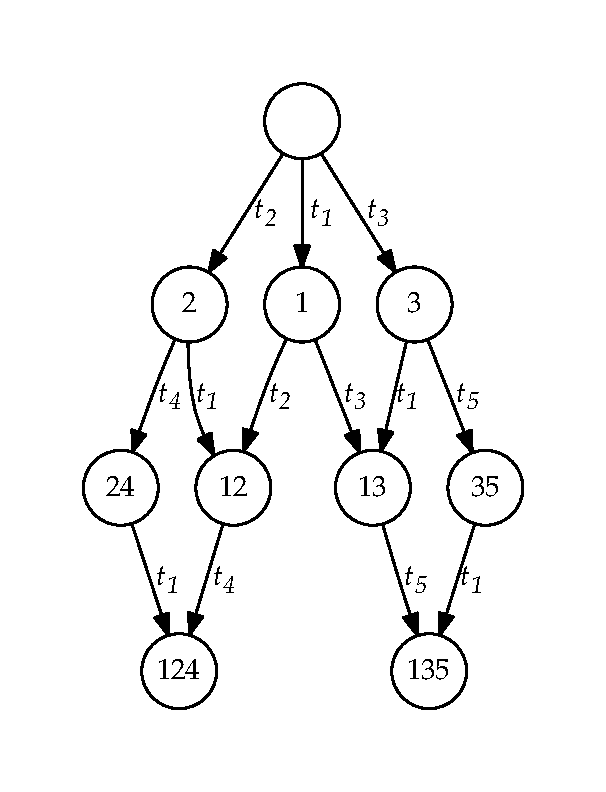
\includegraphics[height=9cm]{persistent1}
	\caption[Diagram of an example state space, for
	the illustration of persistent sets.]
		{Diagram of an example state space, for
		the illustration of persistent sets. Transition
		$t_1$ is independent with the others, which are
		all dependent with one another.}
	\label{fig:persistent}
\end{figure}

\subsubsection{Soundness}
Indeed, it can be shown that if a stopped state is reachable by an exhaustive
search of the state space, then by computing a persistent set $T$ at
each state $\sigma$ and exploring only those transitions from
$\sigma$ that are in $T$, that stopped state is still reachable
\cite[Theorem~4.3]{god96}. It can also be shown
that by exploring only transitions in persistent sets, all reachable
local states of each process are explored
\cite[Theorem~6.14]{god96}. Therefore, if we are interested in
the definition of model checking given in 
Section~\ref{sec:simple-model-checking}, then it is sufficient
to explore transitions from the persistent sets of the states we
encounter.

\subsection{Sleep Sets}
\label{sec:sleep-prep}
Another technique for addressing the state explosion
problem is that of \emph{sleep sets}. Suppose that
we are at state $\sigma_0$ when performing a search
of the state space (see Figure~\ref{fig:sleep}).
Suppose that the first transition
we explore from $\sigma_0$ is $t_1$, reaching $\sigma_1$,
and the second is $t_2$, reaching $\sigma_2$.
If $t_1$ and $t_2$ are independent, then there
is a state $\sigma'$ reachable by both
$\sigma \xrightarrow{t_1} \sigma_1
\xrightarrow{t_2} \sigma'$ and
$\sigma \xrightarrow{t_2} \sigma_2
\xrightarrow{t_1} \sigma'$.
Any stopped state reachable from $\sigma'$
is reachable from $\sigma_1$, as $\sigma'$
is reachable from $\sigma_1$. By assumption,
when the search is at $\sigma_2$, we have already
explored all the stopped states reachable from
$\sigma_1$ (the dotted area in Figure~\ref{fig:sleep}),
in particular those reachable from
$\sigma'$. Therefore, there is no need to
explore $t_1$ from $\sigma_2$.

In fact, there is no need to consider executing
$t_1$ in our recursive exploration from $\sigma_2$
until we execute some transition $t'$ which is
\emph{not} independent of $t_1$, as after
the execution of such a $t'$, exploring $t_1$ may
then lead to an unexplored area of the state space.

A \emph{sleep set} for a particular state
is then the set of transitions which, when
explored, is guaranteed by the above
argument to lead to an already-explored
section of the state space\footnotemark.
\footnotetext{In the literature, sleep
	sets seem to be defined as the sets used
	in the sleep set algorithm, so a
	better definition cannot be given here.}
The technique of
sleep sets is orthogonal to the technique
of persistent sets---there is no interaction
between the two, so implementing
both simultaneously can be achieved with
no extra difficulty.

\begin{figure}
	\centering
	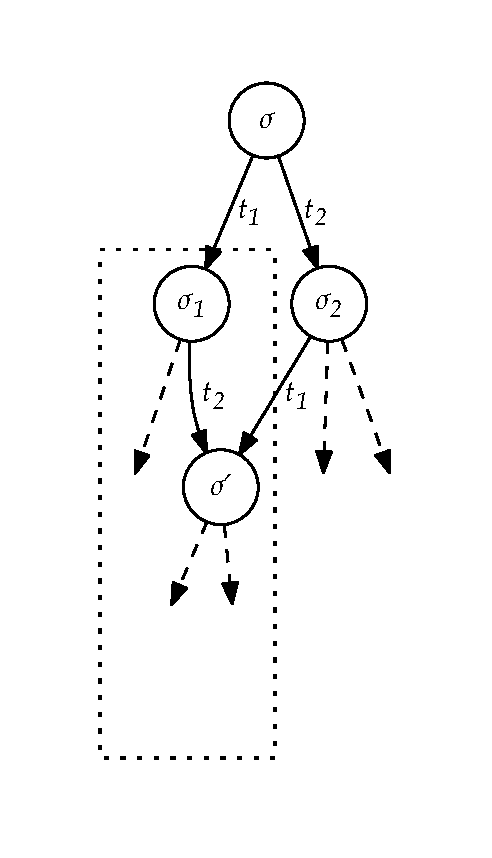
\includegraphics[height=8cm]{sleep}
	\caption{Diagram illustrating of the motivation
		of sleep sets.}
	\label{fig:sleep}
\end{figure}

\section{Dynamic Partial-Order Reduction}
\label{sec:dpor-prep}
Before implementing the dynamic partial-order
reduction algorithm, I first had to
understand how it works.
After reading this section, you should
also understand how the dynamic
partial-order reduction algorithm works.

\subsection{Background Definitions}

\subsubsection{Transition Sequences}
Instead of keeping track of just the current state, as
the algorithms in Section~\ref{sec:simple-model-checking}
did, the dynamic partial-order reduction (DPOR) algorithm
keeps track of a \emph{transition
sequence} $\pi \in \mathcal{T}^*$. This transition
sequence is implicitly executed from the initial state of
the transition system, $\sigma_0$, so that in practice,
$\pi = t_0, t_1, \ldots, t_{n-1}$ determines a sequence of states
$\sigma_0, \sigma_1, \ldots, \sigma_n$ such that
\[
	\sigma_0 \xrightarrow{\ t_0\ } \sigma_1 \xrightarrow{\ t_1\ }
	\ldots \xrightarrow{t_{n-1}} \sigma_n.
\]

Given a transition sequence $\pi = t_0, t_1, \ldots, t_{n-1}$,
we use the following notation:
\begin{itemize}[label={}]
	\newcommand{\defsindent}{3.5em}
	\item{\makebox[\defsindent]{\hfill$\pi_i$}
		--- the transition $t_i$;}
	\item{\makebox[\defsindent]{\hfill$\pi.t$}
		--- the transition sequence $\pi$ extended with
		an additional transition, $t$;}
	\item{\makebox[\defsindent]{\hfill$\textit{dom}(\pi)$}
		--- the set $\{i \in \mathbb{N} \mid 0 \leq i < n \}$;}
	\item{\makebox[\defsindent]{\hfill$|\pi|$}
		--- the length of the transition sequence, $n$;}
	\item{\makebox[\defsindent]{\hfill$\textit{pre}(\pi, i)$}
		--- the state $\sigma_i$ (i.e. the
		state immediately before transition $\pi_i$); and}
	\item{\makebox[\defsindent]{\hfill$\textit{last}(\pi)$}
		--- the final state, $\sigma_n$.}
\end{itemize}

\subsubsection{The Happens-Before Relations}\label{sec:happens-before}

Suppose that two adjacent transitions, $\pi_i$ and $\pi_{i+1}$,
are swapped in a
transition sequence, $\pi$, to give a new
transition sequence, $\pi'$. Suppose further
that $\pi_i$ and $\pi_{i+1}$ are independent.
Since $\pi_{i+1}$ is enabled in $\textit{pre}(\pi, i+1)$,
$\pi_{i+1}$ must also be enabled in $\textit{pre}(\pi, i)$,
as independent transitions cannot disable one another.
If $\pi_{i+1}$
is executed in $\textit{pre}(\pi, i)$,
it results in a state in which $\pi_i$
can be executed, as it cannot be disabled by $\pi_{i+1}$.

Because independent transitions commute, the state reached by
executing $\pi_i$ followed by $\pi_{i+1}$ is the same
as the state reached by executing $\pi_{i+1}$ followed
by $\pi_i$ (see Figure~\ref{fig:sequence-equivalence}).
So $\textit{pre}(\pi, i+2) = \textit{pre}(\pi', i+2)$. Since
for all $j \geq i + 2$, $\pi_j = \pi'_j$, it follows that
$\textit{last}(\pi) = \textit{last}(\pi')$. So swapping
a pair of adjacent transitions results in the same
final state if the swapped transitions are independent.

\begin{figure}
	\centering
	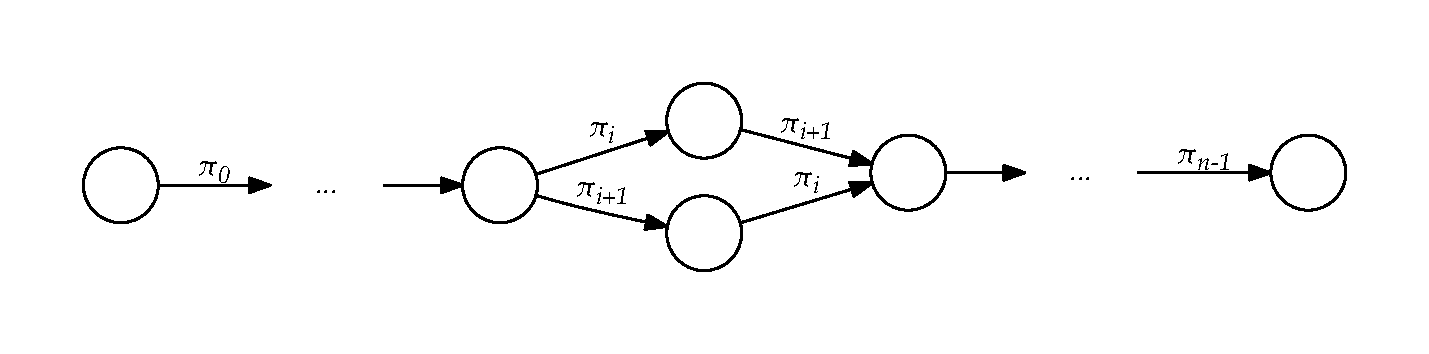
\includegraphics[width=\textwidth]{seqequiv}
	\caption{Illustration of equivalent transition sequences.}
	\label{fig:sequence-equivalence}
\end{figure}

Such equivalent interleavings
of transitions are precisely what we are interested in.
We can think of a transition sequence as representing
the equivalence class of transition sequences obtained
by swapping adjacent pairs of independent transitions;
if we can identify that two transition sequences are
members of the same equivalence class, we need only
explore one.

To help us to reason about such equivalence classes,
we will use a ``happens-before'' relation to identify
when one transition cannot be swapped with another.
In particular, we define the \emph{happens-before}
relation $\longrightarrow_\pi$ for a transition
sequence $\pi$ to be the smallest relation on
$\textit{dom}(\pi)$ such that
\begin{enumerate}
	\item if $i \leq j$ and $\pi_i$ is dependent with
		$\pi_j$ then $i \longrightarrow_\pi j$, and
	\item $\longrightarrow_\pi$ is transitively closed.
\end{enumerate}

By construction, the happens-before relation is a
partial-order relation on the transitions in $\pi$,
and $\pi$ is one of the linearisations of this
partial order. The other linearisations of the
partial order are the equivalent sequences of
transitions which can be obtained by swapping
adjacent pairs of independent transitions in $\pi$.

The DPOR algorithm makes use of a variant of the
happens-before relation.
Informally, if $(i, p)\!\hookrightarrow_\pi$ then
in every linearisation $\hat{\pi}$ of the
happens-before relation (that is, every sequence
obtained by swapping pairs of adjacent,
independent transitions in $\pi$), the next
transition for process $p$ in
state $\textit{pre}(\pi, i)$ is executed
at some point before $\textit{last}(\hat{\pi})$.
Formally, 
if $i \in \textit{dom}(\pi)$ and $p \in
\mathcal{P}$ then we
say that $(i, p)\!\hookrightarrow_\pi$ if
either
\begin{enumerate}
	\item $\textit{proc}(\pi_i) = p$, or
	\item $\exists k \in \textit{dom}(\pi).\;
	i < k \,\wedge\, \textit{proc}(\pi_k) = p
	\,\wedge\, i \longrightarrow_\pi k $.
\end{enumerate}


\subsection{The Dynamic Partial-Order Reduction Algorithm}

\subsubsection{Overview}

The dynamic partial-order reduction algorithm
uses information dynamically gathered during its
exploration of a state space to explore only
transitions in a persistent set from each state
encountered on the search---a partial-order
reduction technique. The idea is that the
extra information which is available because
the persistent sets are created dynamically
allows smaller (and therefore more efficient)
persistent sets to be chosen than an algorithm
computing its persistent sets statically.

In particular, at each state $\sigma$, the
next transition
to execute, $t$, is chosen arbitrarily, and it is
initially assumed that that transition will
be the only transition to be explored from
that state. However, this is a persistent
set only if $t$ is
independent of every transition reachable
by exploring any transitions
from $\sigma$ other than $t$. Clearly,
this is not true in general, so, at each
state $\sigma'$ encountered beyond
$\sigma$, if there is a transition
$t' \in \textit{enabled}(\sigma')$
such that $t'$ is dependent with
$t$, and $t'$ may appear before $t$
in an exploration from $\sigma$, then
a backtracking point is added at
$\sigma$ to ensure that such an
exploration is made.
The addition of such backtracking points
ensures that the set of transitions
explored from each state is a
persistent set.

A detailed explanation of the DPOR
algorithm is given in
Appendix~\ref{app:dpor-walkthrough}.
It is worth emphasising again that
going from having no knowledge of
model checking to
fully understanding this algorithm
took me several weeks
of research and reading.

\newcommand{\dporpseudocode}{
	\begin{algorithmic}[1]
		\Procedure{Explore}{$\pi$}
		\Let{$\sigma$}{$\textit{last}(\pi)$}
		\ForAll{$p \in \mathcal{P}$}
		\State \Call{UpdateBacktrackSets}
		{$\pi,\, \textit{next}(\sigma, p)$}
		\EndFor
		\If{$\textit{enabled}(\sigma) \neq \emptyset$}
		\Let{$t$}{any $t \in \textit{enabled}(\sigma)$}
		\Let{$\textit{backtrack}(\sigma)$}{$\{t\}$}
		\Let{$\textit{done}(\sigma)$}{$\emptyset$}
		\While{$\textit{done}(\sigma)
			 \neq \textit{backtrack}(\sigma)$}
		\Let{$t$}{any $t \in (\textit{backtrack}(\sigma)
			\setminus \textit{done}(\sigma))$}
		\State add $t$ to $\textit{done}(\sigma);$
		\State \Call{Explore}{$\pi.t$}

		\EndWhile
		\EndIf
		\EndProcedure
		\State
		\Procedure{UpdateBacktrackSets}{$\pi,\, t_{p,s}$}
		\Let{$D$}{$\{i \in \textit{dom}(\pi) \mid
			\pi_i \text{ is dependent with } t_{p,s}
			\text{ and } (i, p)\!\not \hookrightarrow_\pi \}$}
		\If{$D \neq \emptyset$}
		\Let{$\sigma_d$}
		{$\textit{pre}(\pi,\text{max}(D))$}
		\If{$\textit{next}(\sigma_d, p)
			\in \textit{enabled}(\sigma_d)$}
		add $\textit{next}(\sigma_d, p)$
		to $\textit{backtrack}(\sigma_d)$
		\Else {
			add all of $\textit{enabled}(\sigma_d)$
			to $\textit{backtrack}(\sigma_d)$
		} \EndIf
		\EndIf
		\EndProcedure
		\State
		\State Initially: \Call{Explore}{$\emptyset$}
	\end{algorithmic}
}

\subsubsection{Example Execution}
An example execution could be added here, on the same example as
Figure~\ref{fig:sdpor-motivation}.

\section{Preparatory Work}
After reading this section, you
should understand exactly what work I
did before beginning the implementation
of the project.

\subsection{Reading}

The main work that was necessary before
I began implementing the project was the
development of a firm understanding of an
area of computer science that was new to me,
and particularly an understanding the DPOR algorithm.
I achieved this by reading the paper that
introduced dynamic partial-order reduction \cite{flan05}
and following
its references to read the literature that
first introduced the various ideas.

\subsection{Requirements Analysis}
Having
understood precisely what properties the
DPOR algorithm can check, I was in a
position to decide exactly what the
finished project should do.
I set out to implement two algorithms:
first, the simple model-checking
algorithm to ensure I was comfortable
with the basics, and then the DPOR
algorithm. I would also need to
implement a simple language which
could be used to express concurrent
programs to model check.

\subsection{Using OCaml}
I implemented the project in OCaml.
However, I had only written very small
programs in SML previously, so I needed to
understand both the differences between
SML and OCaml, and how large programs
are structured using the module system
in OCaml. I achieved both of these
by making use of online resources and
experimenting with small test programs.

\chapter{Implementation}
\label{cha:imp}
After reading this chapter,
you should understand:
\begin{understandinglist}
	\item the software development approach
	I used;
	\item the high-level structure and
	organisation of my project;
	\item the decisions I made
	when designing and implementing
	the programming language used
	as the object language for the
	project; and
	\item the details of my
	implementations of the
	algorithms in the project.
\end{understandinglist}


\section{Software Engineering}
After reading this section, you should
understand how I approached the
development of a project of this
size, and what the high-level
structure of the project software is.

\subsection{Development Strategy}
I used what can be described as an
\textit{incremental} approach to the
development of my project. That is,
I broke the end goal down into
several subgoals, then I effectively
used miniature versions of the waterfall
strategy to implement each subgoal. That
is, for my next target, I would make sure
I knew exactly what the target was, then
I would implement it, and then I would
test it.
I chose this incremental approach
because it allowed me to focus on one
small goal at a time, made it easy for
me to frequently test new components as
they were built, and gradually built up
to a working project.

My first subgoal was to design
a simple programming language and write an interpreter
for it; my next was to design and implement
a concurrent language
by using the sequential language to
specify code for different threads;
my next (which was not in my original plan but
the need for it became apparent) was to write
a parser for the language; next was to implement
the simple model-checking algorithm; and the
last task before reaching the goal was to
implement the DPOR algorithm. I also implemented
each extension as an increment.


\subsection{Structure of the Project}
The project was implemented in OCaml, which
offers a few key advantages:
\begin{itemize}
	\item a clean, functional
	style, which is particularly appropriate for
	this project, given its mathematical nature;
	\item a strong, safe type system, which makes
	impossible a large class of runtime errors;
	\item parametric polymorphism, a module system,
	and other higher-order programming features,
	facilitating abstraction and generalisation; and
	\item established libraries, providing efficient
	implementations of basic data structures and algorithms.
\end{itemize}
I took particular advantage of the module system when
designing and implementing the project. OCaml modules
are used to encapsulate related definitions and hide
information---\emph{signatures} are software interfaces
providing declarations,
and \emph{structures} are implementations which 
provide definitions. A structure \emph{matches} a
signature if it has a definition for each declaration
in the signature. \emph{Functors} can be thought of
as functions from structures matching a
particular signature to structures matching another.

\begin{figure}
	\centering
	\begin{subfigure}{.4\textwidth}
		\centering
		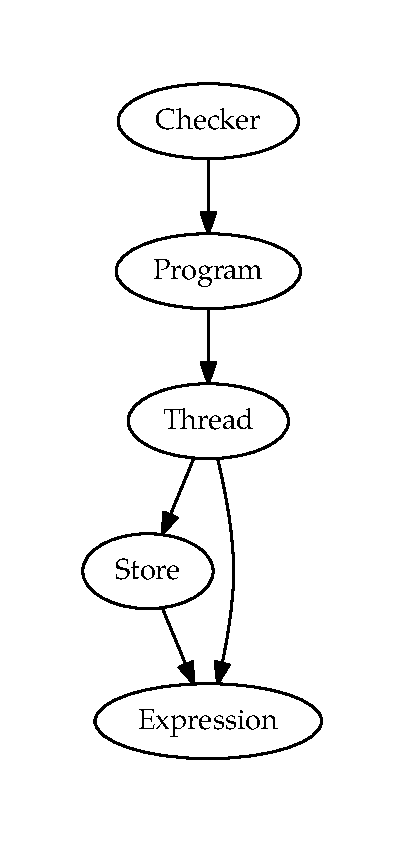
\includegraphics[height=9cm]{interfaces}
		\caption{Diagram showing which signatures declare
			which other signatures as nested sub-structures.}
		\label{fig:interfaces}
	\end{subfigure}%
	\quad
	\begin{subfigure}{.5\textwidth}
		\centering
		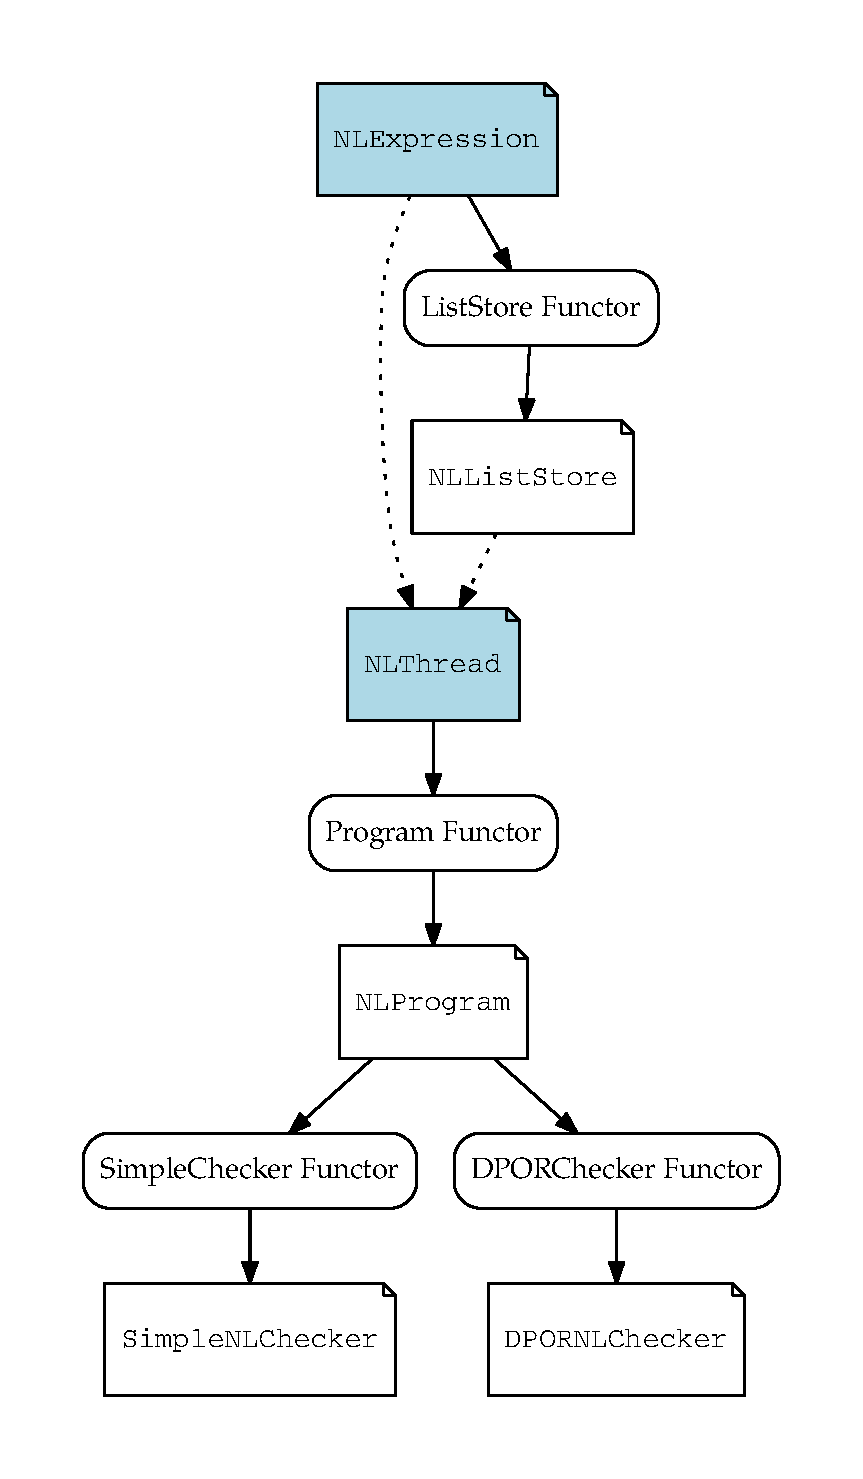
\includegraphics[height=12cm]{functors}
		\caption{Diagram showing generation of
			structures using functors.
			The shaded files must be provided,
			the functors are part of my project,
			and the remaining files
			are generated using the functors.}
		\label{fig:functors}
	\end{subfigure}
	\caption{Diagrams showing the interactions between
		the software modules.}
	\label{fig:design}
\end{figure}

In the project, there are five main signatures:
\begin{enumerate}
	\item a structure that matches \emph{Expression}
	contains information about the structure of expressions
	in the programming language of interest;
	\item a structure that matches \emph{Store}
	implements a mapping from locations
	to expressions for some implementation of \emph{Expression};
	\item a structure that matches \emph{Thread} contains
	the information about the semantics
	of the programming language;
	\item a structure that matches \emph{Program}
	contains declarations relating to
	transition systems as expressed in some programming
	language; and
	\item a structure that matches \emph{Checker}
	contains a function which performs model checking.
\end{enumerate}

While I did implement a simple programming language
(see Section~\ref{sec:language}), the model checking
algorithms that are the focus of this project are of
course entirely independent of any particular language.
I therefore ensured that, in order to use
my project to perform model checking for programs
in any other language, the work that would have to
be done would be minimal. In particular, given implementations
of \emph{Expression} and \emph{Thread} (effectively
specifying the syntax and semantics of a programming
language), my system uses
functors to automatically generate implementations of
\emph{Store}, \emph{Program} and \emph{Checker}, the
last of which can then be used to immediately perform
model checking. This process is shown explicitly in
Figure~\ref{fig:functors} for
a hypothetical language called NL.

\section{Development of the Project Language}
\label{sec:language}
After reading this section, you should
understand how I designed
and implemented the programming
language in which the programs to
be model checked are written.

\subsection{Language Design}
Although, as mentioned above, any concurrent
thread-based programming language
could be used to express transition systems for model
checking, I chose to design and implement a simple
ML-like language, PL (Project Language), to avoid
the unnecessary complexity of implementing a full
industrial language.
The grammar for valid PL expressions is given in
Figure~\ref{fig:pl-expressions}.

As required by the \emph{Thread} interface, each
PL thread has access to both its local store
$s$\footnote{Note that
	here, $s$ is not the full local state
	as defined in Chapter~\ref{cha:prep},
	because it does not include the instructions
	for the thread. An (expression, store) pair
	gives the full local state.}
and the shared store $g$. Both $s$ and $g$ are
maps from locations to expressions.
To express the semantics
of PL, then, we need to decide whether an
expression $e$ reduces for local store $s$ and
global store $g$, and if it does, we need to give
the expression $e'$ that it reduces to in one ``step'',
as well as any updates to $s$ and $g$ that result.
Each such step is assumed to be atomic, so care
must be taken to ensure that each step really is
atomic, else race conditions could exist that would
not be found by a model checker.
The semantics of PL expressions are as you would expect
(see Appendix~\ref{app:pl-def} for a full definition), but
the rules for the reduction of expressions that interact
with the global store $g$ are given in Figure~\ref{fig:pl-rules}.

There is no type system for PL. Although it would have been
beneficial to design and implement a type system for PL
(a type checker could catch type errors early, rather than a runtime
failure with non-obvious causes occurring), I thought that the total
time I would have spent on creating the type system would be more than
the time taken in dealing with the problems resulting from having
no type system. With the benefit of hindsight, I think this was the
correct decision.

\subsection{Parser}
On the other hand, I decided that investing time in creating a
parser for PL would pay itself off over the course of the project.
A parser allowed me to write, for example,
\begin{align*}
	\texttt{let y = ref 1 in cas(Gx, 7 * !y - 3, 0)},
\end{align*}
instead of having to type the OCaml meta-language abstract
syntax tree representing the structure of the PL expression:
\begin{align*}
	\texttt{Let (Ref (Integer}& \texttt{ 1), Cas (Global "x",
		Op (Op (Integer 7,} \\ \texttt{Mult,}& \texttt{ Deref (Var 0)), Minus, Integer 3),
		Integer 0))}.
\end{align*}
Writing such expressions is not only extremely time-consuming but
also error-prone. For the language to be of any practical use,
a parser was a necessity.

To create a parser for PL, two program generators were used:
OCamllex and Menhir. When presented with a
file giving a mapping from strings of characters to tokens,
OCamllex produces a lexical analyser, which converts a sequence
of characters into a sequence of tokens. When presented with a
grammar and a set of precedence rules, Menhir produces a parser,
which converts a sequence of tokens into an abstract syntax tree
of the grammar. These were used in conjunction, as shown in
Figure~\ref{fig:parsing}, to produce a full PL parser.

\begin{figure}
	\centering
	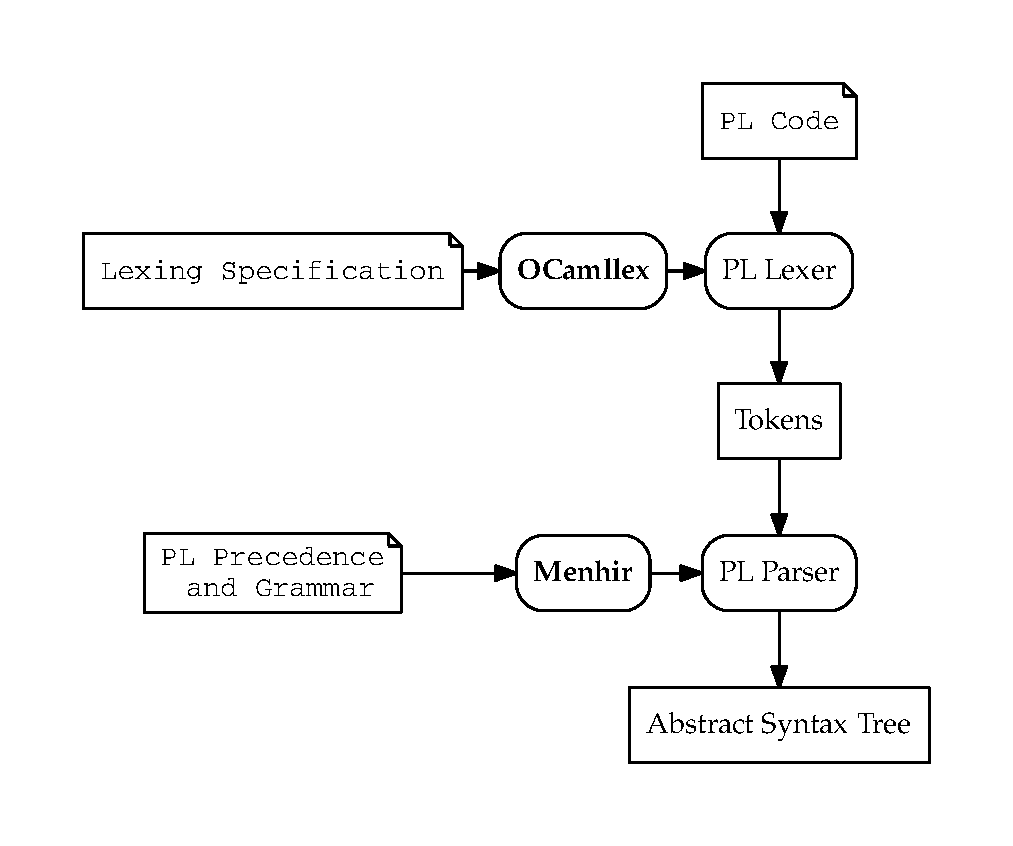
\includegraphics[height=10cm]{parsing}
	\caption{Diagram showing the flow and processing of
		information in the generation of a PL abstract
		syntax tree.}
	\label{fig:parsing}
\end{figure}

\subsection{Implementation}

\subsubsection{The Expression Module}
There are actually two datatypes which are used to
represent PL expressions: the ``raw'' expression, which
uses strings to represent variables (this is the
datatype that the parser produces), and a datatype
which uses De Bruijn indices \cite{debr72} to
represent variables, allowing
easier manipulation of expressions.

The remainder of the \emph{Expression} module
consists mainly of auxiliary functions which are
necessary for the implementation of later
modules, and either return a simple piece
of information or perform a simple manipulation.

\subsubsection{The Store Module}
As mentioned above, I implemented a functor
called ListStore, which takes an
\emph{Expression} implementation and
gives a \emph{Store} implementation, which
represents stores using lists of
(location,~expression) pairs. Mappings
are introduced by adding a new pair to
the front of the list, causing any old
mapping for that location to become stale.
A function is provided that walks through
the list removing stale pairs, used to
prevent the list from growing too long,
or in situations when there must be
no stale values in the list.

More efficient store implementations are of
course possible (for example, one based on
a hash table rather than a list), but
I decided on the simplest reasonable
implementation I could think of, to
be confident of its correctness.

There are again various auxiliary functions
used in implementing later modules.

\subsubsection{The Thread Module}
The \emph{Thread} module consists primarily of
the \texttt{next\_step} and \texttt{next\_transition}
functions, which define the semantics of PL.
Given an expression, \texttt{next\_step} uses pattern
matching to determine what the next atomic
operation (if any) is for the reduction
of that expression. Given the definition
of a transition (cf.\@ Section~\ref{sec:trans-prep}),
the \texttt{next\_transition}
function repeatedly calls the \texttt{next\_step}
function until some step accesses the shared
store, at which point the resulting expression
and updates to the stores are returned.

\subsubsection{The Program Module}
The \emph{Program} module is a small functor which,
when given a \emph{Thread} implementation, provides 
the few additional definitions and auxiliary
functions necessary to fully represent the state of
transition systems (cf.\@ Section~\ref{sec:background-defs}).
In particular, a state $\sigma \in \textit{State}$ is
represented by an instance of the \texttt{state} type:
\lstinputlisting[frame=none, firstline=121, lastline=121]
	{../src/interfaces.ml}

\subsubsection{Testing}
To ensure that the implementation of the PL
language was correct, I wrote around twenty unit tests for
the \texttt{next\_transition} and
\texttt{next\_step} functions. These had good
code coverage, and seemed to catch most of the bugs
in the implementation of PL.


\section{Dynamic Partial-Order Reduction}
The dynamic partial-order reduction (DPOR)
algorithm was presented in Section~\ref{sec:dpor-prep},
which gave an overview of its operation,
including high-level pseudocode, which is reproduced
in Figure~\ref{fig:dpor-imp-pscode} for ease
of reference. Several
aspects of the algorithm mean that it
is not obvious how it can be implemented
as an executable program; after reading
this section, you should understand
how this was achieved.

\subsection{Implementation}
This section gives a
line-by-line explanation of how the algorithm
was implemented.
For a line-by-line explanation of how the algorithm
works, see Appendix~\ref{app:dpor-walkthrough}.

\begin{figure}
	\dporpseudocode
	\caption{The DPOR pseudocode}
	\label{fig:dpor-imp-pscode}
\end{figure}

\begin{description}
	\item[Line 1] The \textsc{Explore} procedure
	is implemented as a recursive OCaml function,
	\texttt{check}.
	One of the advantages of OCaml is its provision
	of practical procedural features, as well the
	functional ML features, which usefully allowed
	me to combine these styles as I saw fit when
	implementing this algorithm.

	\item[Line 2] When implementing the simple
	model checker, I used the \texttt{fold\_left}
	function from the provided List module to
	repeatedly use the \texttt{apply\_transition}
	from the \textit{Program} module to apply
	the transitions in the transition sequence
	to the initial state. However, in this case
	I wrote a function, \texttt{pre},
	which applies only the first
	$n$ transitions in the sequence,
	thereby returning the state
	$\textit{pre}(\pi, n)$ if $n < |\pi|$
	or the state $\textit{last}(\pi)$ if
	$n = |\pi|$, which is what we want in
	this case.

	\item[Lines 3--4] The \texttt{next\_transition}
	function, provided in the \textit{Thread} module,
	may return no transition at all (for instance
	in the case that a thread has terminated its
	computation), so the call to 
	\textsc{UpdateBacktrackSets} is only made if
	\texttt{next\_transition} does return a
	transition. It is also here, in the
	iteration through the threads,
	that it is decided whether the current
	state is an error or a deadlock
	(see Section~\ref{sec:dpor-imp-detecting}
	below).

	\item[Lines 15--17] In this project,
	the assumptions are made that
	each transition $t$ accesses only one shared
	object, denoted $\alpha(t)$,
	and that two transitions are
	dependent if and only if they access
	the same shared object (or belong to the
	same process). Therefore, the most
	recent transition $\pi_i$, if any, such that
	$\pi_i$ is dependent with $t_{p,s}$
	and $(i,p)\!\not\hookrightarrow_\pi$,
	is precisely the last transition
	to access the shared object that
	$t_{p,s}$ accesses.

	Therefore, as well as the transition
	sequence, $\pi$, \texttt{check} takes
	as an argument 
	a function $L$ from shared objects to
	the index of the last transition that
	accessed them, so that the index of the
	necessary backtracking point, if any, is
	$L(\alpha(t_{p,s}))$. However, this
	is not a necessary backtracking point if
	$\pi_{L(\alpha(t_{p,s}))}$ happens-before
	$t$, in which case no backtracking point
	is necessary, as there cannot be another
	transition that is dependent with $t$
	but does not happen-before $t$. To
	decide the happens-before relation,
	clock vectors are used, as described 
	in Section~\ref{sec:clock-vectors}.

	The \texttt{pre} function mentioned above is used to
	obtain $\sigma_d$ from the index of the
	transition executed from it, $L(\alpha(t_{p,s}))$.

	\item[Lines 18--19]	The \texttt{next\_transition} function
	returns a Boolean with each transition, indicating whether
	it is enabled in the given state, so that deciding if
	$\textit{next}(\sigma_d,p)$ is enabled is trivial.
	This also
	means it is easy to compute the enabled
	set of a state, by iterating through the processes
	and looking at whether the next transition of each
	is enabled.

	\item[Lines 5--6] If, while iterating through the
	processes in lines 3 and 4, any transition is found to be
	enabled, then a reference is set to it. If at line 5,
	that reference has been set at all, then it is chosen
	as the $t \in \textit{enabled}(\sigma)$ in line 6,
	otherwise lines 6 to 12 are not executed.

	\item[Line 7] The \textit{backtrack} sets for each state
	in the sequence of states implied by the transition
	sequence $\pi$ must be stored in a data structure that
	allows them to be accessed and updated from all later
	recursive calls, so that they can add backtracking
	points. I decided to use a variable-length array
	for this, as arrays are mutable and have efficient
	access, but the maximum recursion depth (and so the
	longest fixed-length array necessary) cannot be predicted.
	
	I therefore implemented a module which uses a fixed-length
	array to implement a variable-length array by
	copying the elements to a fresh array of double the
	previous size if the underlying array proves too short.
	Although this operation is expensive, the amortised
	cost of adding a new element to the array is constant.
	In this case, each element of the array is a \textit{backtrack}
	set of a state, implemented as a list of processes
	whose next transitions are to be explored.
	
	\item[Lines 8--11] Instead of using a
	procedural while-loop,
	I implemented the iteration through
	the backtracking points
	by using a functional tail-recursive
	function, whose argument
	was a list of processes, representing
	the \textit{done} set. An auxiliary
	function returned a member $p$ of the
	\textit{backtrack} set not present in the
	\textit{done} set, from which the
	transition $t$ to explore is simply
	$\textit{next}(\sigma, p)$. The
	recursive call to the while-function
	then has the old \textit{done} set
	extended with $p$ as its argument. If
	the auxiliary function can
	find no such $p$, then the
	while-function (and therefore the
	call to \texttt{check}) returns.

	\item[Line 12] Once the new arguments have
	been computed, a recursive call to
	\texttt{check} is made. Other than
	the clock vectors (see Section~\ref{sec:clock-vectors}),
	the arguments that
	have to be computed are the new transition
	sequence, $\pi' = \pi.t$,
	and the new function, $L'$,
	tracking which transitions accessed each 
	object:
	\[ L'(o) =
	\begin{cases}
		\hfill |\pi| \hfill & \text{ if } o = \alpha(t); \\
		\hfill L(o) \hfill & \text{ otherwise}.
	\end{cases}\]
	As the transition sequence is implemented as an
	OCaml list, and the function $L$ as an OCaml function,
	these computations are straightforward.

	\item[Line 13] Once all backtracking points have been
	explored, the result is returned.
	Appendix~\ref{sapp:simple-code} explains
	exactly how errors and deadlocks are
	detected in the simple model checker,
	and the computation is very similar
	for the DPOR algorithm. The iteration
	through all threads on line 3 is used
	to also check whether any thread has
	encountered an error, is enabled,
	or is blocked.
	These results are combined with the
	results from the recursive calls to
	return the correct result.

\end{description}

\subsection{Deciding The Happens-Before Relation}
\label{sec:clock-vectors}

To decide the happens-before relation,
$\hookrightarrow_\pi$, I used the method
of clock vectors, as outlined by Flanagan
and Godefroid \cite{flan05}.

\subsubsection{Using Clock Vectors}

As explained above, although
the last function, $L$, gives the index
of the last transition that accessed a given shared
object, and so the index of the potential backtracking
point to be added, we only need to add it if it
didn't happen-before the current transition.
That is, if
$(L(\alpha(t_{p,s})), p)\!\not\hookrightarrow_\pi$.


If, for each process
$q$, we know the index $k$ of the last transition of that
process such that $(k, p)\!\hookrightarrow_\pi$,
then given any other transition of
process $q$, $\pi_i$, we know that
$(i, p)\!\hookrightarrow_\pi$ if and only if
$i \leq k$. A clock vector $c$ is
a function from processes $q$ to such
indices into the transition sequence, $k$,
and we maintain one clock vector, $c_p$, per
process $p$. To decide whether
$(i, p)\!\hookrightarrow_\pi$ for
any $i$ and $p$, is simply to decide
whether $i \leq c_p(q)$, where $q$ is
the process of transition $\pi_i$.

\subsubsection{Updating Process Clock Vectors}
By passing clock vectors as arguments to
\texttt{check}, then, it is straightforward
to decide whether
$(L(\alpha(t_{p,s})), p)\!\hookrightarrow_\pi$.
For this to work, the correct clock values need
to be passed to each call of \texttt{check}.
Assuming that the correct value is passed for
the initial call,
(each $k$ set to anything less than 0)
we need to ensure that the
clock vectors are correctly updated when
making a recursive call, when a new
transition, $t_{p,s}$, is being explored.

The only clock vector that needs to be updated
is $c_p$, the clock vector for the process
of the transition being explored, because
a transition of process $p'$ must happen-before
the end of the extended transition
sequence, $\pi' = \pi.t_{p,s}$, if and
only if it must happen-before the end
of the original transition sequence,
$\pi$, assuming that $p' \neq p$.

Let us denote the updated clock vector
by $c_p'$, and consider $c_p'(q)$, which
must be at least $c_p(q)$, as if process
$p$ must happen-before the end of $\pi$
then it must happen-before the end of $\pi'$.
However, if there is a more recent transition
of process $q$, say $\pi_i$
that accesses the same shared
object as the new transition $t_{p,s}$, then
$c_p'(q)$ must be updated to the index of
that transition, because $\pi_i$ must
happen-before $t_{p,s}$.

To perform this update, we need to keep
track of the index $k$ of the most recent
transition of each process $p$ that
accesses each shared object $o$. We therefore
also maintain a clock vector $c_o$ for each
shared object $o$, and set
\[ c_p'(q) =\textit{max}(c_p(q),
		c_{\alpha(t_{p,s})}(q)).\]
The only special case is when $q = p$,
in which case $c_p'(p) = |\pi|$, since
the last transition is now a transition of
process $p$, and $|\pi|$ is the index
of the last transition in $\pi'$. The
full update for the clock vector is therefore
\[ c_p'(q) =
\begin{cases}
	\hfill |\pi| \hfill & \text{ if } q = p; \\
	\hfill \textit{max}(c_p(q),
		c_{\alpha(t_{p,s})}(q))
		\hfill & \text{ if } q \neq p.
\end{cases}\]


\subsubsection{Updating Object Clock Vectors}

We have seen how to use object clock vectors to
update the process clock vectors, but of course
the object clock vectors themselves must be
updated whenever a new transition is explored.
In particular, if the clock vector for the
object accessed by the transition must be
updated so that the thread of the transition
maps to that transition:
\[c_{\alpha(t_{p,s})}'(p) = |\pi|.\]

However, we can do better, by letting
$c_o(q)$ be the index of the
last transition of process
$q$ such that object $o$ is guaranteed to be
accessed between $c_o(q)$ and the last
transition of the sequence (inclusive),
whether or not $\pi_{c_o(q)}$ itself
accesses $o$.
This is sufficient for updating the
process clock vectors as above, and
also allows for higher indices to
be stored than just the last
transition of a process that
accesses the object.

For example, suppose that,
for some process $q \neq p$,
$c_{\alpha(t_{p,s})}(q) < c_p(q)$. That is,
more recently than the last transition of
$q$ that accessed the object $\alpha(t_{p,s})$,
there was a transition of $q$ that happens-before
some transition of process $p$ prior to the new
transition $t_{p,s}$. Since any previous
transition of process $p$ must happen-before
$t_{p,s}$, we know that the transition
of index $c_p(q)$ must also happen-before
$t_{p,s}$. Therefore, there is a transition
(namely $t_{p,s}$) which
accesses $\alpha(t_{p,s})$ and is guaranteed
to happen after $\pi_{c_p(q)}$. So we can
safely perform the following update:
\[ c_{\alpha(t_{p,s})}'(q) =\textit{max}(c_p(q),
c_{\alpha(t_{p,s})}(q)),
\]
meaning that the full update for the object
clock vector is

\[ c_{\alpha(t_{p,s})}'(q) =
\begin{cases}
\hfill |\pi| \hfill & \text{ if } q = p; \\
\hfill \textit{max}(c_p(q),
c_{\alpha(t_{p,s})}(q))
\hfill & \text{ if } q \neq p.
\end{cases}\]

Noting that this is precisely the same
clock vector as $c_p'$ allows for a
more efficient implementation of
the updates.

\section{Counter-Example Traces} \label{sec:traces}
One of the advantages of model checking
is that, if
an error is found, it is easy to
give an example execution leading
to that error---in
our case, this is just the sequence of
transitions leading to the error state.
To give more insight into the reason for the
error state being entered, the user could
instead be given a
\emph{partial order} of the transitions which,
whenever linearised into an execution,
results in the error (or deadlock) state.

This partial order is simply the happens-before
relation, as described in
Section~\ref{sec:happens-before}. As
two transitions are dependent if and only
if they belong to the same thread or if
they access the same shared object, my
algorithm simply executes the given transition
sequence, using functions from processes
and shared objects to positions in
the sequence to track the last
transition to each process and
to access each shared object respectively.
For each
transition executed, two ``happens-before''
edges are added
to the graph representing the partial
order: one from the last transition
belonging to the same process, and one
from the last transition accessing the
same shared object.

I thought that displaying the partial
order visually would be easiest to
understand, so I wrote a procedure which
automatically outputs the graph as
a GraphViz file, with each node
labelled with its process and the
shared object it accesses.
GraphViz is an open-source program which
draws graphs.
Figure~\ref{fig:trace-example} gives a program
and shows an example of such an
automatically-generated GraphViz graph.

\begin{figure}
	\centering
	\begin{subfigure}{0.5\textwidth}
		\centering
		\begin{tabular}{l}
			Shared variables: \\
			\qquad \texttt{n}, \texttt{w},
			\texttt{x} and \texttt{y},
			initially \texttt{0} \\
			\qquad \texttt{t} and \texttt{z},
			initially \texttt{false} \\
			\\
			Thread 0: \\
			\qquad \texttt{t := z;} \\
			\qquad \texttt{if t then x := y} \\
			\\
			Thread 1: \\
			\qquad \texttt{n := 1;} \\
			\qquad \texttt{z := true} \\
			\\
			Thread 2: \\
			\qquad \texttt{y := 2;} \\
			\qquad \texttt{if w = 1 \& x = 2 then \textbf{error}} \\
			\\
			Thread 3: \\
			\qquad \texttt{w := n} \\
			\\
			Thread 4: \\
			\qquad \texttt{t := false} \\
		\end{tabular}
	\end{subfigure}%
	\begin{subfigure}{0.5\textwidth}
		\centering
		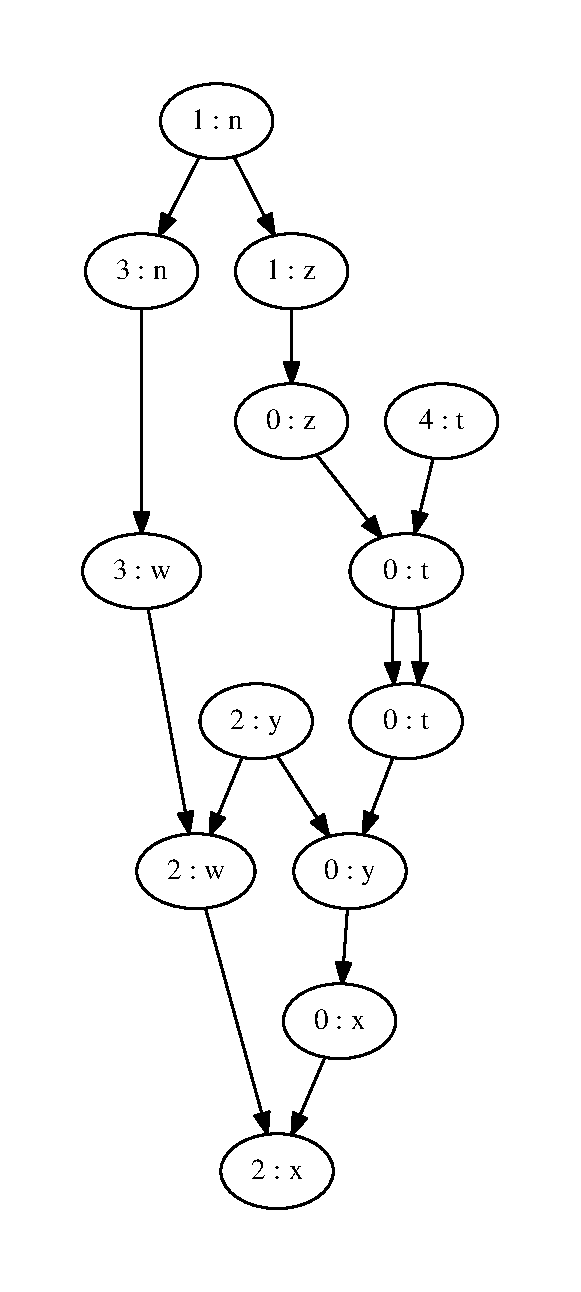
\includegraphics[height=15cm]{error_trace}
	\end{subfigure}
	\caption[An example partial-order
	error trace.]{An example partial-order
		error trace. The assignments in
		the program are implemented in PL
		using compare-and-swap operations.}
	\label{fig:trace-example}
\end{figure}

\section{Extensions For Evaluation}
Having reached my goal of implementing
the DPOR algorithm, I decided to
implement some additional model-checking
algorithms as extensions, to allow a
comparative evaluation of their
performances. After reading this
section, you should understand how
I implemented these other model-checking
algorithms.

\subsection{Simple Model Checker}
I actually implemented and tested
the simple
model checker before the DPOR
algorithm, to allow me to
sanity-check my PL implementation
and to later verify
that my DPOR implementation
gave correct results.
As outlined in
Section~\ref{sec:simple-model-checking}, it
performs an exhaustive depth-first
search of the state space,
recursively deciding whether each
state is error-free
and deadlock-free.
Appendix~\ref{app:pseudocode} gives
the pseudocode for this algorithm,
and shows how it is decided whether
an error or deadlock state has been reached.

\subsection{Stateful Model Checking}
If we keep track of which states we have
already explored on a search, then when
we re-encounter a state, we can cut short
the search in the knowledge that we have
already explored from that state, improving
time efficiency at the cost of extra space.

\subsubsection{Simple Model Checker}

Applying this technique to the simple model
checking algorithm is straightforward: whenever
a state is visited, add it to some data structure,
then explore only those states which are not
present in that data structure. As querying
this structure and inserting a state to it
happens at almost every state, we would like these
operations to be efficient. The typical amortised costs
of these operations for a hash table are both
constant, so I used the OCaml library implementation
of hash tables for this purpose.

\subsubsection{Dynamic Partial-Order Reduction}

Suppose that we applied this approach
to the DPOR algorithm,
and executed the resulting algorithm
on the example shown in
Figure~\ref{fig:sdpor-motivation}.
Consider the stage at which
all the states in grey have been
explored and so are present in the hash table,
and the current transition sequence is the first
transition of thread 1 followed by the first
transition of thread 0. As this stage, the state
labelled 2200 is encountered, which is already
present in the hash table, so no exploration is
made, and as no backtracking points have been added
at either of the previous stages, the algorithm
terminates.

However, this leaves part of the state
space entirely unexplored (the dotted section in
the diagram), meaning that the algorithm is unsound;
any error or deadlock in a dotted state would go
undetected.
The reason for the unsoundness is the failure to
introduce backtracking points when necessary. If the
search had not been cut short, then a backtracking point
would have been added in the second state (1200), causing the
dotted section to be explored.

Solving this by simply adding
all possible backtracking points
whenever the search is cut short turns out to
give worse performance than plain DPOR.
To use this technique,
we need a method of conservatively deciding which
backtracking points must be added for soundness, but not
so conservatively that all practical benefits are lost.

\begin{figure}
	\begin{subfigure}{\textwidth}
		\begin{tabular}{lp{1cm}lp{0cm}l}
		Shared variables: &&Thread 0: &&Thread 1: \\
		\qquad \texttt{m} and \texttt{n}, initially \texttt{1}
			&&\qquad\texttt{m := 2;}
			&& \qquad\texttt{n := 2;} \\
		\qquad \texttt{x} and \texttt{y}, initially \texttt{0}
			&&\qquad\texttt{x := n}
			&& \qquad\texttt{y := m}
		\end{tabular}
	\end{subfigure}
	\begin{subfigure}{\textwidth}
		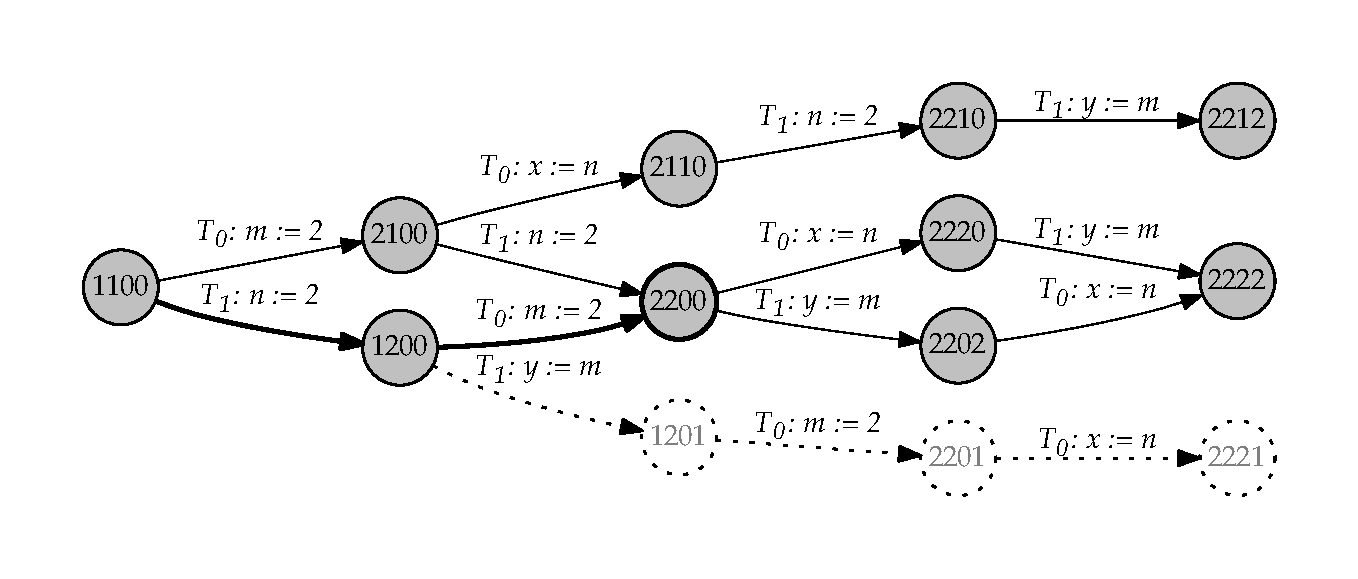
\includegraphics[width=\textwidth]{sdpor}
	\end{subfigure}
	\caption[An example illustrating the need for the
		Stateful DPOR algorithm.]
		{An example showing that na\"{\i}vely
		cutting short the DPOR algorithm is
		unsound. Each state in the diagram shows
	the values of \textit{mnxy}.}
	\label{fig:sdpor-motivation}
\end{figure}

\subsubsection{Stateful Dynamic Partial-Order Reduction}

One such method is to use a \emph{visible operation dependency
graph}, proposed by Yang et al.\@ in an
algorithm known as stateful dynamic
partial-order reduction (SDPOR) \cite{yang08}.
The idea is that, when we first explore
a section of the state space,
we make a note of the visible operations
that may be executed, so that if we encounter that section again,
we can cut short the search, and use our knowledge of the
visible operations that may have been
executed if the search was continued
to add backtracking points as necessary.

In particular, a \emph{visible operation dependency
graph} is a graph $G = \langle V, E \rangle$ whose
nodes represent visible operations, and whose edges
represent the ordering of those transitions; whenever
a transition sequence of the form
$\sigma_1 \xrightarrow{t} \sigma_2 \xrightarrow{t'}
 \sigma_3$
is encountered in a search of the state space, the
edge $(t, t')$ is added to the visible operation
dependency graph $G$. Then, when a state $\sigma$ is
encountered which has already been explored on the
search, sufficient backtracking points for soundness
can be added by calling the
\textsc{UpdateBacktrackSets} procedure
on each transition in the set
\[\mathcal{U} = \{u \mid \exists t \in \textit{enabled}(\sigma).\;
   u \text{ is reachable from node } t \text{ in graph } G\}.\]
For its efficiency, SDPOR relies on the assumption that
the sets $\mathcal{U}$ of reachable transitions
are generally small in size.

The pseudocode for the SDPOR algorithm is shown
in Appendix~\ref{sapp:sdpor-code}.
To implement the visible operation dependency graph
$G$, I chose to use another hash table,
mapping from transitions to lists of transitions.
Calling \textsc{UpdateBacktrackSets} on
each reachable node in $G$ is implemented using
a simple depth-first search.

\subsection{Static Partial-Order Reduction}
\label{sec:spor-imp}

In order to evaluate the improvement in performance
allowed by building persistent sets dynamically
instead of statically, I decided to research and
implement a static partial-order reduction
algorithm. However, I struggled to find one
in the literature that I could
understand and implement in the short amount
of time I had. I therefore designed my own
rudimentary static partial-order reduction algorithm,
which I will refer to as the static partial-order reduction
(SPOR, not to be confused with SDPOR) algorithm.
While it is easy to understand and implement,
the trade-off is that it returns large persistent sets.

The algorithm explores the state space using a
depth-first search, but exploring only those
transitions in a persistent set from each
state, as outlined in section \ref{sec:persistent}.
Before the algorithm begins its search, it compiles a table
listing all the shared objects that each process may
access, then, during the search, persistent sets $T$ are
constructed such that
every process whose next transition is
not in $T$ never accesses any
object that any process whose next
transition is in $T$ accesses.
The pseudocode for this algorithm is
given in Appendix~\ref{sapp:spor-code}.

This algorithm assumes that every thread only
accesses shared objects mentioned in its own
local state, as opposed to being communicated
through the shared state, giving it a more
limited scope than the other model-checking
algorithms I implemented.

My initial idea was to compute the objects that
each thread could access at every state encountered.
While this would result in marginally smaller
persistent sets as the threads progress, the cost
of performing this expensive computation at
every state was prohibitively high.


\subsection{Sleep Sets}

To implement sleep sets, as
explained in Section~\ref{sec:sleep-prep},
I adapted my
code for the simple model-checking
algorithm to match the pseudocode
given in Appendix~\ref{sapp:sleep-code}.
As usual, I used a
library hash table implementation,
and used lists of process identifiers
to represent sleep sets, since one
integer takes up much less memory
than one representation of a transition,
while providing sufficient information
for this purpose.

Applying the sleep-set technique to the
dynamic partial-order reduction
algorithm involves keeping track of the
sleep sets in the same way, and never
adding backtracking points for
processes that are in the sleep set
of the relevant state. This is
sound, although not as obviously as
it might first seem \cite{flan05addm}.

\chapter{Evaluation}
\label{cha:evaluation}

After reading this chapter,
you should understand:
\begin{understandinglist}
	\item the extent to which I believe
	my project is correct, and the evidence
	motivating that belief;
	\item why being certain of the
	correctness of a model checking
	system is not essential for it
	to be of practical use;
	\item how the model-checking
	algorithms I implemented perform
	in comparison to one another,
	in terms of the reduction in the
	size of the explored state space; and
	\item how my implementations
	of the model-checking algorithms
	perform, in terms of their
	execution times.
\end{understandinglist}

\section{Soundness}

Even though the algorithms
used in this project have all been proven sound,
this is irrelevant if there are bugs in my
implementations which render the algorithms incorrect.
After reading this section, you should
therefore understand the extent to which I believe
my project consists of sound implementations
of the model-checking algorithms, the
evidence leading to this belief, and why
model checking systems are useful in
practice without being known to be
sound.

\subsection{Evidence for Soundness}
Any program of a reasonable size is very
likely to contain bugs. Industry average
is about 1 to 25 errors per 1,000 lines
of delivered code \cite{mccon04}, my project
consists of at least 3,250 lines of
code\footnote{Computed using
	\texttt{\,find src/ -name
		\textquoteleft*.ml\textquoteright
		| xargs wc -l}},
and there is no reason to think that I would
produce fewer errors than the average
professional software developer.
However, I believe that
on the balance of probabilities,
all remaining bugs in my project
are likely to relate
to functionality not necessary for
soundness. For instance, I would
not be surprised to learn that there
is a bug in the \texttt{next\_transition}
function for PL, whereas I would be
surprised if such a bug existed in
my implementation of the DPOR
algorithm. There are two main reasons
for this belief: my review and understanding
of the code, and my testing process.

\subsubsection{Review of Source Code}
OCaml is a very high-level language, so
its use allowed me to keep the source code
relatively simple. As a result,
the correspondence between
the published pseudocode for an algorithm
and my source code implementing it is
relatively simple, meaning that it
is possible to greatly increase
your confidence that
the implementation is correct by simply
comparing the two. In the development
process, I spent a lot of time trying
to find ways in which my programs did
not match the pseudocode; at the end
of the development process, I can be
reasonably confident that any significant differences
in semantics have been found.
This is especially
true for the simple model checker,
due to its lack of complexity.

\subsubsection{Tests}
\label{sec:pl-checker-tests}
As part of the development process,
I wrote over forty varied test cases, each
consisting of a transition system
implemented as a PL program, and
the expected
$(\textit{error-free},\, \textit{deadlock-free})$
result of model checking that program.
Running an implementation of a
model-checking algorithm on the
program should give the expected
result: if not, then either
the result I expected was wrong
(usually due to an incorrect encoding
of the transition system in PL),
or the implementation was incorrect.
To ensure the former was not a possibility,
I used the simple model checker---whose
correctness I have confidence in---to check that my
expectations of the results were correct.

The primary use of these tests was to
reveal the presence of bugs in my
project during its development, so
that I could track them down and
remove them. However, they have the
secondary benefit of providing
evidence that my implementations are
correct: if a bug is not applicable
in any of the test cases, then,
assuming that these test cases cover a
varied and representative selection
of systems to be verified,
the bug must be obscure.

\subsection{Model Checking In Practice}
Even if I think it unlikely, it is
certainly possible that there is a subtle
bug in my project which results in its
unsoundness, since my project has not
been verified (verification of such
large programs takes
considerable effort).
Although it may initially seem
that a model-checking system without
a guarantee of its
soundness is useless, this
is not at all the case.

Proof can be seen as a social process
by which a consensus arises that
a statement is true, and it has been
argued that, compared to the informal
proofs typically used in mathematics,
formal proofs are a
poor catalyst to this process, since
they are so long and difficult to
read \cite{demi79}. There are other
ways that the confidence in a program's
correctness can be increased, which
are arguably better at convincing people, including
running tests, gaining experience from
long-term use, and especially performing
cross-checking with other, ideally
independently developed, implementations
\cite{tau02}.

There are also more important factors
which determine the practical use of
verification systems, including their
performance and usability. A system that
catches 90\% of bugs can still be a
useful tools, especially if it catches
those which are difficult to expose
using conventional testing, such as
those caused by race conditions. On
the other hand, if a system
is guaranteed to be sound, but takes an
impractically long time for any realistic
program, or if it requires users to have
weeks of training and a deep mathematical
understanding, then it will not be used in
practice.
Similarly, a system that
returns only a single Boolean result
is much less useful than one such as my project,
which can give information indicating where
the problem lies in the event that the
program does not meet its specification.

Perhaps the clearest indication of the
practical value of unverified
model-checking systems is in their widespread
practical use and resulting successes.
\cite{kur08, brat04, est12, kars96, cof10, mill08}
It is also worth noting that, as of 2006,
there were only
two verified model checking
systems, neither of which was widely
used, despite model
checking having been in use for
over two decades \cite{beck06}.


\section{Performance}
After reading this section, you should
understand how the different
model-checking algorithms compare to
one another in terms of reduction in
state space explored,
how efficient my implementations of
them are, and how these two aspect
combine to result in the observed execution
times.

\subsection{Methodology}
Unfortunately, there is no concurrent program
that is ``typical'' for verification by model
checking. I have therefore had to pick some
example programs for which to analyse the performance
of my project. For each of these programs, I varied
some test parameter---normally the number of threads
used---and recorded for each algorithm
both the number of (not necessarily unique) transitions
explored, which is a measure of how successful
the algorithm is in addressing the state
explosion problem for the given case, and also
the execution time, which is really the bottom
line.

The four programs I picked were:
\begin{enumerate}
	\item the simplest example program I could think of, where
	each thread repeatedly accesses the same location
	for no reason,
	to see how the algorithms behaved in this special
	case;
	\item a solution to the bounded-buffer problem,
	with one producer and one consumer, to see how
	the algorithms performed in this well-known
	and useful example;
	\item the ``Indexer'' example used in the paper
	that introduced dynamic partial-order reduction \cite{flan05},
	to allow comparison with the published results, and
	to see how DPOR behaves when the conditions are
	favourable; and
	\item the ``File System'' example from the same paper,
	for the same reasons.
\end{enumerate}

The number of transitions for each algorithm was easily
obtained by counting the number of recursive calls made.
The execution times were measured using the \texttt{time}
function in the Sys module packaged with OCaml. It returns
measurements of time only in quanta of 0.004 seconds,
so the accuracy of the time measurements is not good for
executions of under around 0.04 seconds.
The precision of measurements
is good, though, with very similar results being returned
for multiple executions of the same program.
having established this,
I therefore took only one measurement
of each execution time, preferring
to collect more data on different examples than to collect
redundant data on the same example.

\subsection{Results}
This section presents the performance measurements.
For each example program, the results for all eight
algorithms are plotted on the same graph, in the
style indicated in Figure~\ref{fig:key}.
As the results are
presented on logarithmic graphs, if the timing function
returned 0s, I plotted a point at 0.02s
to represent the fastest possible execution, since
$\log(0)$ is undefined.

If an algorithm failed to terminate after around
100 seconds, I abandoned its execution,
resulting in incomplete data
for some algorithms in some cases.

\begin{figure}
	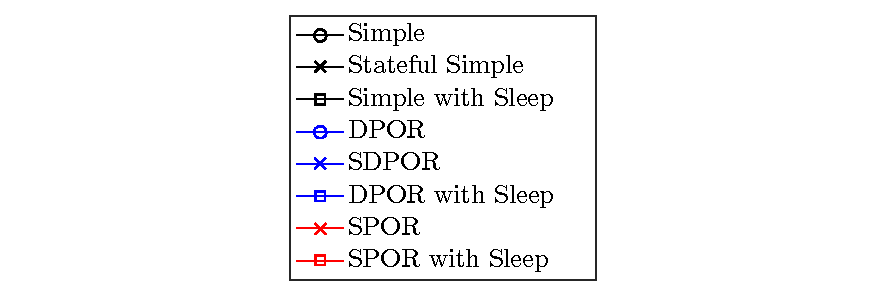
\includegraphics[width=\textwidth]{key}
	\caption[Key for algorithm performance graphs.]
	{Key for algorithm performance graphs.
		Rather than reproduce the key on each graph,
		it is given just once, here.}
	\label{fig:key}
\end{figure}

\subsubsection{Example 1 -- Repeated Accesses}
Each thread in this example is assigned a particular
shared object, and simply accesses this object a
fixed number of times. There are three test parameters:
the number of threads, the number of threads that are
assigned to access the same shared object, and the fixed
number of accesses to the shared object that each thread
makes. If, for example, these were set to 6, 2 and 5
respectively, then threads 0 and 1 would access object A,
threads 2 and 3 would access object B and threads 4 and 5
would access object C, and each thread would make 5 accesses
to its assigned object. This allows a controlled amount of
dependence between the threads -- if each thread has its own
object, then all transitions are independent; if all threads
access the same object, then all transitions are dependent.

\begin{figure}
	\centering
	\footnotesize
	\begin{figtile}
		\input{figs/t43_tpl1_ops1.pdf_tex}
		\caption{1 thread per object,
			each making 1 access.}
	\end{figtile}%
	\quad
	\begin{figtile}
		\input{figs/t43_tpl1_ops3.pdf_tex}
		\caption{1 thread per object,
			each making 3 accesses.}
	\end{figtile}
	\begin{figtile}
		\input{figs/t43_tpl2_ops1.pdf_tex}
		\caption{2 threads per object,
			each making 1 access.}
	\end{figtile}%
	\quad
	\begin{figtile}
		\input{figs/t43_tpl2_ops3.pdf_tex}
		\caption{2 threads per object,
			each making 3 accesses.}
	\end{figtile}
	\begin{figtile}
		\input{figs/t43_tpl3_ops1.pdf_tex}
		\caption{3 threads per object,
			each making 1 access.}
	\end{figtile}%
	\quad
	\begin{figtile}
		\input{figs/t43_tpl3_ops3.pdf_tex}
		\caption{3 threads per object,
			each making 3 accesses.}
	\end{figtile}
	\begin{figtile}
		\input{figs/t43_tpl4_ops1.pdf_tex}
		\caption{4 threads per object,
			each making 1 access.}
	\end{figtile}%
	\quad
	\begin{figtile}
		\input{figs/t43_tpl4_ops3.pdf_tex}
		\caption{4 threads per object,
			each making 3 accesses.}
		\label{fig:repeated-access-trans-h}
	\end{figtile}
	\caption{Numbers of transitions
		explored for the repeated-accesses example.}
	\label{fig:repeated-access-trans}
\end{figure}

\begin{figure}
	\centering
	\footnotesize
	\begin{figtile}
		\input{figs/t43_time_tpl1_ops1.pdf_tex}
		\caption{1 thread per object,
			each making 1 access.}
	\end{figtile}%
	\quad
	\begin{figtile}
		\input{figs/t43_time_tpl1_ops3.pdf_tex}
		\caption{1 thread per object,
			each making 3 accesses.}
	\end{figtile}
	\begin{figtile}
		\input{figs/t43_time_tpl2_ops1.pdf_tex}
		\caption{2 threads per object,
			each making 1 access.}
	\end{figtile}%
	\quad
	\begin{figtile}
		\input{figs/t43_time_tpl2_ops3.pdf_tex}
		\caption{2 threads per object,
			each making 3 accesses.}
	\end{figtile}
	\begin{figtile}
		\input{figs/t43_time_tpl3_ops1.pdf_tex}
		\caption{3 threads per object,
			each making 1 access.}
	\end{figtile}%
	\quad
	\begin{figtile}
		\input{figs/t43_time_tpl3_ops3.pdf_tex}
		\caption{3 threads per object,
			each making 3 accesses.}
	\end{figtile}
	\begin{figtile}
		\input{figs/t43_time_tpl4_ops1.pdf_tex}
		\caption{4 threads per object,
			each making 1 access.}
	\end{figtile}%
	\quad
	\begin{figtile}
		\input{figs/t43_time_tpl4_ops3.pdf_tex}
		\caption{4 threads per object,
			each making 3 accesses.}
		\label{fig:repeated-access-time-h}
	\end{figtile}
	\caption{Execution times for the repeated-accesses example.}
	\label{fig:repeated-access-time}
\end{figure}

\subsubsection{Example 2 -- Bounded Buffer}
This example is the classic bounded-buffer problem,
in which two threads operate on a shared fixed-length
array of items, with one thread ``producing'' items
and writing them to the buffer and the other
``consuming'' them and removing them from the buffer.
In this example program, the buffer is of size 8,
race conditions are prevented by using a lock per
item to effect mutual exclusion, and the number
of items that the threads produce and consume is
the test variable.

\begin{figure}
	\centering

	\def\svgwidth{\textwidth}
	\input{figs/prod_cons_trans_fig.pdf_tex}
	\caption{Numbers of transitions explored
		for the bounded-buffer example.}
	\label{fig:prod-cons-time}
	\def\svgwidth{\textwidth}
	\input{figs/prod_cons_time_fig.pdf_tex}
	\caption{Execution times for the
		bounded-buffer example.}
	\label{fig:prod-cons-trans}
\end{figure}

\subsubsection{Example 3 -- Indexer}
This example is taken from
the paper that introduced DPOR,
where the code can be seen \cite[Figure~1]{flan05}.
Each thread ``receives'' a number of
``messages'' from a \texttt{getmsg}
procedure, each of which is inserted
into a shared hash table. If the
hash table slot is already taken, the
next free slot is used instead.

\begin{figure}
	\centering

	\def\svgwidth{\textwidth}
	\input{figs/indexer_trans_fig.pdf_tex}
	\caption{Numbers of transitions explored
		for the indexer example.}
	\label{fig:indexer-trans}

	\def\svgwidth{\textwidth}
	\input{figs/indexer_time_fig.pdf_tex}
	\caption{Execution times
		for the indexer example.}
	\label{fig:indexer-time}
\end{figure}

\subsubsection{Example 4 -- File System}
This example is taken from
the paper that introduced DPOR,
where the code can be seen \cite[Figure~7]{flan05}.
Based an idiom found in the Frangipani file
system \cite{thek97}, each thread searches for a free
``disk block'' for an ``inode'' to point
to. Mutual exclusion is again achieved using
locks.

\begin{figure}
	\def\svgwidth{\textwidth}
	\input{figs/fs_trans_fig.pdf_tex}
	\caption{Numbers of transitions explored
		for the file-system example.}
	\label{fig:fs-trans}

	\def\svgwidth{\textwidth}
	\input{figs/fs_time_fig.pdf_tex}
	\caption{Execution times
		for the file-system example.}
	\label{fig:fs-time}
\end{figure}

\subsection{Performance of the Algorithms}

\subsubsection{Simple Model Checker}
As expected, the simple model checker performs
consistently poorly, with the size of the state
spaces explored increasing exponentially as
the number of threads increase (seen most
clearly in Figure~\ref{fig:repeated-access-trans})
and as the amount of work done by each thread
increases (seen most clearly in
Figure~\ref{fig:prod-cons-trans}).
This is the state explosion problem.

\subsubsection{Stateful Simple Model Checking}
By looking at Figure~\ref{fig:repeated-access-trans},
we can see that the stateful model checker does
explore fewer transitions than the stateless
algorithm. The benefit offered increases
when there are more operation per threads,
which is because each time a state is
revisited and therefore not re-explored,
a bigger saving is made.

The benefit also increases when there are more
threads sharing each shared object, which I
believe is due to a quirk in my implementation
of stores: because I implemented stores as
(\textit{object}, \textit{value}) lists,
and updates simply
add a new pair to the start of the list,
if two updates are made to a store, the
results stores will only be equal in
the eyes of OCaml if the updates are
identical, regardless of whether the
stores are logically equivalent or not.

To resolve this quirk, I should use
my own equality function on states,
rather than using the inbuilt
OCaml structural quality operator.
This would result in more
revisited states being spotted.

\subsubsection{Dynamic Partial-Order Reduction}
When all threads are independent of one another,
as in the first two cases of
Figure~\ref{fig:repeated-access-trans},
the DPOR algorithm explores only one path
through the state space, because no
backtracking points are ever added as
no race conditions can exist. The total
transitions explored in this case is linear in both
number of threads and number of operations
per thread, which is considerably better
than the exponentially increasing costs
of the simple algorithm.

In the other cases in
Figure~\ref{fig:repeated-access-trans},
when a new thread is added, the increase
in transitions explored
is either additive (with negligible cost),
or multiplicative (with considerable cost).
The increase is additive if the new thread
is assigned to access a new shared object,
in which case no new race conditions are
added, so no new backtracking points are
necessary. The increase is multiplicative
if the new thread accesses the same shared
object as a number of existing threads
(and the increase is more severe the greater
this number is), since at many states, there
now could be a new race condition, since
two threads access the same shared object,
so more backtracking points are needed.
The increase is not as severe as in the
simple algorithm, though, because the new
thread is independent of at least some of
the threads (unless the number of threads
is no more than the number of threads
per shared object).

In the bounded-buffer example
(Figure~\ref{fig:prod-cons-trans}),
the DPOR algorithm is able to exploit
the independence between the two threads
(they are only dependent when they
access the same item out of eight) to
reduce the exponent in the
exponential cost caused by the
state explosion problem.

The remaining two examples were created
by their authors specifically to show
off the benefits of the DPOR algorithm.
As such, it performs very well up to
a certain number of threads in both cases,
being able to exploit independence that can
only be known with dynamic runtime information,
before the number of threads becomes high enough
that they are no longer independent, and the
exponential increase begins, albeit at a lesser
rate than that of the simple algorithm.
Incidentally, the similarity of these performance
graphs and those shown in the paper introducing
dynamic partial-order reduction \cite{flan05}
is further evidence that the algorithm has
been correctly implemented -- the shapes
are identical, and the numerical
differences can be explained by the
translation of the example into PL.

\subsubsection{Stateful Dynamic Partial-Order Reduction}
In every case presented above, the SDPOR algorithm
explores at least as many transitions as the DPOR
algorithm, and in some cases many more. I can think
of four possible explanations for this behaviour:
\begin{enumerate}
	\item the `quirk' that worsened the performance
	of the simple stateful model checker causes
	much more serious problems for SDPOR; or
	\item I have misunderstood SDPOR, and
	accidentally implemented an algorithm similar
	to SDPOR which is sound but inefficient; or
	\item the SDPOR algorithm generally does \emph{not}
	give better performance than the DPOR algorithm; or
	\item the SDPOR generally \emph{does} give better
	performance than the DPOR algorithm, but by
	coincidence does worse on the examples I chose.
\end{enumerate}
The paper introducing SDPOR compared its performance
with that of DPOR against five benchmarks \cite{yang08},
which suggests that the third reason is less likely.
The fact that one of these benchmarks is an instance
of the bounded-buffer problem (albeit one that
has multiple producers and consumers rather than
just one of each) suggests that the fourth reason
is also less likely. The first reason is certainly
possible: it could be that by failing to notice
when some states are revisited, the algorithm's
advantages are lost, leaving only its substantial
costs.
The second reason is also possible:
while I can not see where any
misunderstanding is, I can accept that it is
a reasonable explanation for the very poor
performance of SDPOR in my project.

\subsubsection{Sleep Sets}
Sleep sets can be seen to be a consistently
effective technique for reducing the number
of transitions explored. In every example,
sleeps sets significantly reduce the
severity of the exponential increase in
the number of transitions explored by the
simple algorithm, by preventing the
unnecessary re-exploration of sections
of the state space that have already been
covered (and is considerably more effective
at this than the simple stateful algorithm).

When applied to the DPOR algorithm, the results
are more variable. No benefit whatsoever is seen
in Figure~\ref{fig:repeated-access-time} and little
is seen in Figure~\ref{fig:indexer-trans},
presumably because the DPOR algorithm has already
exploited the independence of the transitions
as fully as is possible. However, in
Figure~\ref{fig:prod-cons-trans}, sleep sets
work in conjunction with the DPOR to greatly
slow the rate of the exponential increase,
and in Figure~\ref{fig:fs-trans} at fourteen and
more threads, sleep
sets slow the rate of increase to a reasonable
rate, whereas the loss of independence at the
fourteenth thread meant that DPOR alone took too long
to terminate.

As well as combination with DPOR allowing
sleep sets to reduce the number of states
(as opposed to just transitions) explored,
Flanagan and Godefroid note that
\begin{quote}
	There is a nice complementarity between sleep sets and our
	dynamic partial-order reduction algorithm: when a process
	$q$ is introduced in $\textit{backtrack}(\textit{pre}(\pi, i))$
	\textellipsis \ because
	of a potential conflict between $i$ and
	$\textit{next}(\sigma, p)$, there
	is no point in executing $\pi_i$ following
	$\textit{next}(\textit{pre}(\pi, i), q)$ before
	$\textit{next}(\sigma, p)$ is executed;
	this optimization is captured exactly
	by sleep sets. \cite{flan05}
\end{quote}

\subsubsection{Static Partial-Order Reduction}
When every thread accesses separate objects,
then my SPOR algorithm returns persistent sets
of size one, which leads to the minimal number
of transitions being explored, as shown in the
first two cases of
Figure~\ref{fig:repeated-access-trans}.
Otherwise, my SPOR algorithm offers only
small reductions in the number of transitions
explored, the benefits of which increase with
the number of operations per thread.

However, the benefits decrease as
the number of threads sharing each object
increase, because the persistent sets
computed are bigger. In most practical
programs, threads are unlikely to be
able to be partitioned such that
partitions access disjoint sets of objects,
so in most practical situations, my SPOR
algorithm will offer no benefits. This is
the case for the bounded-buffer, indexer
and file-system examples, so I have omitted
the SPOR results from those graphs.
The main benefit of attempting to implement
an SPOR algorithm was a greater understanding
of the complexities involved in trying to
compute a reasonably small persistent set
using only static information.

\subsection{Efficiency of the Implementations}
\subsubsection{Simple Model Checker}
The simple model-checking algorithm takes
constant time (per thread) per transition
explored, so its execution times are
proportional to the number of transitions it
explores. Due to the state explosion problem,
this by far dominates the time complexity.

\subsubsection{Stateful Simple Model Checking}
Although, as notes above, using stateful model
checking offers a small reduction in the number
of transitions explored compared with the simple
algorithm, in practice the overhead of having
to perform hash table operations at every state
mean that the execution times end up being
generally no shorter. Notably, the one
case where stateful checking offers a noticeable
improvement in execution time is that shown in
Figure~\ref{fig:repeated-access-time-h},
suggesting that perhaps in bigger, more
industrial-scale cases, it gives more of
an advantage. It is difficult to confirm
or reject this hypothesis from the other three examples,
because the executions very quickly take too
long to measure.

\subsubsection{Dynamic Partial-Order Reduction}
Theoretically, the DPOR does a fixed amount of
work per thread per transition, including some
memory operations to keep track of the backtrack
sets. As the number of transitions explored
varies with
the number of threads much more than the amount
of work per transition explored does, I would
expect the execution times to be more or less
proportional to the numbers of transitions
explored. The fact that this is what can be
seen in all four examples suggests that my
implementation correctly implements the
algorithm in the sense that it is not more
complex than it needs to be.

\subsubsection{Stateful Dynamic Partial-Order Reduction}
The execution times for the SDPOR algorithm
are both much worse than the DPOR execution
times and much worse than what might be
expected from looking at the number of
transitions explored. This can be
seen particularly clearly in figures
\ref{fig:indexer-time} and \ref{fig:fs-time},
in which the execution times of the SDPOR
algorithm get exponentially worse, despite
the linearly-increasing numbers of
transitions explored. This again
suggests that I might not have
correctly implemented the algorithm.

As well as introducing SDPOR, Yang et al.\@
also introduced a light-weight
scheme for capturing the local states of
threads (based on storing only changes
to the stores, rather than the full stores
every time), to be used in conjunction with
SDPOR. Although I decided not to
implement this for time reasons,
it should not affect the correctness
of SDPOR, nor the numbers of transitions
is explores, and I would be surprised
to learn that not using this technique
was the main reason that the SDPOR
execution times are so long. 

\subsubsection{Sleep Sets}
The overhead costs associated with implementing
sleep sets for the simple model checker
mean that the multiplicative
increases in execution times are slightly
higher than the multiplicative increases
in number of explored transitions. The
benefits of using sleep sets are still
profound, though.

In the repeated-accesses example,
sleep sets do not reduce the number
of explored transitions when applied
to DPOR, so the overhead costs of
implementing sleep sets can be clearly
seen in Figure~\ref{fig:repeated-access-time}.
However, in the other examples, these
small costs are insignificant compared
to the considerable benefits of using sleep
sets.

\subsubsection{Static Partial-Order Reduction}
The extra work done at per transition
in implementing my SPOR
algorithm is deliberately little
(see Section~\ref{sec:spor-imp}), so
execution times are more or less proportional
to the number of transitions explored.

\chapter{Conclusions}

\section{Successes}

As well as meeting the aims of the
project ahead of schedule, I also
managed to implement several
extensions, allowing an
interesting quantitative
comparison of various
model-checking algorithms
and partial-order techniques.
I also gained experience of
reading relatively dense academic
writing, learnt the skill of
translating such writing into
executable programs, and
improved my understanding
of how theoretical developments
in computer science affect the
everyday realities of the
software industry.

Perhaps most importantly,
I am glad I decided on the
project that I did, and
I have (mostly) enjoyed
developing a significant
software system independently
for the first time.

\section{Potential Extensions}
Instead of assuming that any
two processes that access the
same object must be dependent,
it is possible to distinguish
between reads and writes to
shared object, allowing
two reads to be identified
as independent.
Flanagan and Godefroid suggest
that this could be implemented
by keeping two clock vectors per
shared object---one for reads and
the other for writes \cite{flan05}.
It would
be interesting to implement
this algorithm and evaluate its
performance in relation to the
algorithm I implemented.

It would also be interesting
to use my system to check
programs written in a widely-used
language. As mentioned previously,
the only work necessary for this
is implementations of my
\textit{Expression} and
\textit{Thread} signatures.

Dynamic partial-order reduction
was introduced in 2005. It would
be interesting to research,
implement and evaluate more
recent developments.

%%%%%%%%%%%%%%%%%%%%%%%%%%%%%%%%%%%%%%%%%%%%%%%%%%%%%%%%%%%%%%%%%%%%%
% the bibliography
\addcontentsline{toc}{chapter}{Bibliography}
\bibliography{refs}

%%%%%%%%%%%%%%%%%%%%%%%%%%%%%%%%%%%%%%%%%%%%%%%%%%%%%%%%%%%%%%%%%%%%%
% the appendices
\appendix

\chapter{Explanation of the DPOR Algorithm}
\label{app:dpor-walkthrough}
\dporpseudocode
\begin{description}
	\item[Lines 1--2] The \textsc{Explore} procedure implements
	dynamic partial-order reduction. The transition sequence
	$\pi$ which is passed as its argument implicitly specifies the state
	from which the exploration is to take place, $\sigma$.

	\item[Lines 3--4] First, any necessary backtracking points
	which can be identified from this state are added to the
	\textit{backtrack} sets of previous states. Backtracking
	points can be identified using information from each possible
	transition from this state, so the \textsc{UpdateBacktrackSets}
	procedure is called with each possible next transition as an
	argument.

	\item[Line 5] Having updated the \textit{backtrack} sets
	of previous states, the search continues its exploration,
	but only if there are any enabled transitions to explore.

	\item[Lines 6--8] The recursive exploration proceeds by
	maintaining two sets of transitions: \textit{backtrack}
	and \textit{done}. The \textit{backtrack} set contains
	those transitions from $\sigma$ which should be explored,
	and is initialised to contained any single enabled transition.
	Recursive calls to
	\textsc{Explore} may add more transitions to \textit{backtrack}.
	The \textit{done} set contains those transitions
	in \textit{backtrack} that have been explored.

	\item[Line 9] The search from $\sigma$ halts when every
	transition that needs to be explored (is in \textit{backtrack})
	has been explored (is in \textit{done}).

	\item[Lines 10--12] If there is some transition that needs
	exploring, \textsc{Explore} is recursively called with that
	transition extending the current transition sequence $\pi$,
	and that transition is added to \textit{done}.

	\item[Line 14] The \textsc{UpdateBacktrackSets} procedure
	can use the information that a given transition, $t_{p,s}$ can be
	executed in $\sigma$ to add necessary backtracking points.

	\item[Line 15] The set $D$ contains the indices $i$ of the
	transitions $\pi_i$ in the sequence such that $\pi_i$ and
	$t$ are dependent, and $(i, p)\!\not \hookrightarrow_\pi$.
	This second condition means that $t_{p,s}$ is \emph{not}
	guaranteed to happen after $\pi_i$, so $D$ is the set
	of transitions which may have a race condition with
	$t_{p,s}$.

	\item[Line 16] If there are no transitions which have
	a race condition with $t_{p,s}$, then no backtracking
	points need to be added: as far as we know from $t_{p,s}$,
	if we had chosen any other
	choices of transitions to explore previously, we would
	have ended up with a transition sequence in the same
	equivalence class as $\pi$.

	\item[Line 17] If there are transitions in $\pi$
	which have a race condition with $t_{p,s}$, then
	it is sufficient to add a backtracking point at
	the state immediately before
	the most recent of these;
	the necessary backtracking
	points for the earlier states will be added
	by later (or previous) calls of \textsc{Explore}.

	\item[Line 18] We know there is a race condition
	between $t_{p,s}$ and $\textit{next}(\sigma_d,p)$, so
	we want to explore another transition sequence from
	$\sigma_d$ in which $\textit{next}(\sigma_d,p)$
	appears before $t_{p,s}$. If $\textit{next}(\sigma_d,p)$
	is enabled in $\sigma_d$, then we certainly explore such
	a transition sequence by immediately exploring
	$\textit{next}(\sigma_d,p)$ from $\sigma_d$.

	\item[Line 19] However, if we cannot immediately
	explore $\textit{next}(\sigma_d,p)$
	from $\sigma_d$ because it is not enabled, then it is
	not obvious which transitions to explore from $\sigma_d$
	to achieve
	a transition sequence in which $\textit{next}(\sigma_d,p)$
	appears before $t_{p,s}$. The algorithm presented here
	does not attempt to narrow down which transitions might
	lead to such a transition sequence, and instead plays it
	safe and explores them all.

	\item[Lines 21] To perform model checking, the state space
	is explored from the initial state, $\sigma_0$, which is
	reached from $\sigma_0$ by executing no transitions, so
	\textsc{Explore} is initially called on the empty
	sequence of transitions, $\emptyset$.

\end{description}

\chapter{Extension Model-Checking Algorithms}
\label{app:pseudocode}
\section{Simple Model Checker}
\label{sapp:simple-code}
\begin{algorithmic}[1]
	\Procedure{Check}{$\sigma_0,\,\pi$}
	\Let{$(l, g)$}
	{$\textit{last}(\pi)$}
	\Let{\textit{error\_free}}{true}
	\Let{\textit{is\_enabled\_thread}}{false}
	\Let{\textit{no\_waiting\_threads}}{true}
	\Let{\textit{calls\_deadlock\_free}}{true}
	\ForAll{$p \in \mathcal{P}$}
	\If{$\textit{next}(\sigma, p) \in \textit{enabled}(\sigma)$}
	\State \textit{is\_enabled\_thread} := true;
	\Let{$(\textit{result\_ef}, \textit{result\_df})$}
	{\Call{Check}{$\sigma_0, \pi.\textit{next}(\sigma, p)$}}
	\State \textit{error\_free} := \textit{error\_free}
	\& \textit{result\_ef};
	\State \textit{calls\_deadlock\_free}
	:= \textit{calls\_deadlock\_free}
	\& \textit{result\_df}
	\Else
	\If{$\textit{err}(l(p))$}{ \textit{error\_free} := false};
	\EndIf
	\If{$\exists g' \in \mathcal{G}.\;
		\textit{next}(\sigma,p) \in \textit{enabled}(l,g')$}
	{\textit{no\_waiting\_threads} := false}
	\EndIf
	\EndIf
	\EndFor
	\Let{\textit{deadlock\_free}}{\textit{calls\_deadlock\_free} \&
		(\textit{is\_enabled\_thread} | \textit{no\_waiting\_threads})}
	\State \Return (\textit{error\_free}, \textit{deadlock\_free})
	\EndProcedure
\end{algorithmic}

The algorithm assumes that if a thread
encounters an error, then the execution
of that thread will not proceed, meaning
that only threads which do not have any
enabled transitions need to be checked
for errors. The Boolean \textit{error\_free}
is set to false if an error is encountered
either in this state (line 14) or in a
recursive call (line 11).

Deciding whether the state space from the current
state onwards is deadlock-free is more complicated.
The \textit{calls\_deadlock\_free} keeps track of
whether any recursive call reports a deadlock (line 12).
The current state is not a deadlock state
if either there is some thread with an
enabled transition,
or every thread had terminated its computation and
is not waiting for some change in the shared state.
If any transition is enabled, then
\textit{is\_enabled\_thread} is set to true (line 9).
If any thread without an enabled transition is
waiting for some change in the shared state (for
instance a lock to become available), then
\textit{no\_waiting\_threads} is set to false.
These results are combined in line 17.

\section{Stateful Dynamic Partial-Order Reduction}
\label{sapp:sdpor-code}
\begin{algorithmic}[1]
	\Let{$H$}{an empty hash table of states}
	\Let{$G$}{an empty graph on transitions}
	\State
	\Procedure{Explore}{$\pi$}
	\Let{$\sigma$}{$\textit{last}(\pi)$}
	\If{$\sigma \in H$}
	\Let{$\mathcal{U}$}
	{$\{u \mid \exists t \in \textit{enabled}(\sigma).\;
		u \text{ is reachable from node }
		t \text{ in } G\}$}
	\ForAll{$t \in \mathcal{U}$}
	\Call{UpdateBacktrackSets}
	{$\pi,\, t$}
	\EndFor
	\Else{
		\State add $\sigma$ into $H$;
		\ForAll{$p \in \mathcal{P}$}
		\Call{UpdateBacktrackSets}
		{$\pi,\, \textit{next}(\sigma, p)$};
		\EndFor
		\If{$\textit{enabled}(\sigma) \neq \emptyset$}
		\Let{$t$}{any $t \in \textit{enabled}(\sigma)$}
		\Let{$\textit{backtrack}(\sigma)$}{$\{t\}$}
		\Let{$\textit{done}(\sigma)$}{$\emptyset$}
		\While{$\textit{done}(\sigma)
			\neq \textit{backtrack}(\sigma)$}
		\Let{$t$}{any $t \in (\textit{backtrack}(\sigma)
			\setminus \textit{done}(\sigma))$}
		\State add $t$ to $\textit{done}(\sigma)$;
		\If{$|\pi| > 0$}
		add edge $(\pi_{|\pi|-1}, t)$ to $G$;
		\EndIf
		\State \Call{Explore}{$\pi.t$}
		\EndWhile
		\EndIf
	}\EndIf
	\EndProcedure
	\State
	\Procedure{UpdateBacktrackSets}{$\pi,\, t_{p,s}$}
	\Let{$D$}{$\{i \in \textit{dom}(\pi) \mid
		\pi_i \text{ is dependent with } t_{p,s}
		\text{ and } (i, p)\!\not \hookrightarrow_\pi \}$}
	\If{$D \neq \emptyset$}
	\Let{$\sigma_d$}
	{$\textit{pre}(\pi,\text{max}(D))$}
	\If{$\textit{next}(\sigma_d, p)
		\in \textit{enabled}(\sigma_d)$}
	add $\textit{next}(\sigma_d, p)$
	to $\textit{backtrack}(\sigma_d)$
	\Else {
		add all of $\textit{enabled}(\sigma_d)$
		to $\textit{backtrack}(\sigma_d)$
	} \EndIf
	\EndIf
	\EndProcedure
	\State
	\State Initially: \Call{Explore}{$\emptyset$}
\end{algorithmic}
\newpage
\section{Static Partial-Order Reduction}
\label{sapp:spor-code}
\begin{algorithmic}[1]
	\Procedure{PersistentSet}{$\sigma$}
	\Let{$E$}{$\{p\}$,
		for any $p$ such that
		$\exists t_{p,s} \in \textit{enabled}(\sigma)$}
	\Let{$O$}{$\{o \mid \textit{accesses}(p, o)\}$}
	\While{$E$ changes}
	\ForAll{$q \in (\mathcal{P} \setminus E)$}
	\If{$\exists o \in O.\;
		\textit{accesses}(q,o)$}
	\State $E := E \cup \{p\}$;
	\State $O := O \cup \{o \mid
	\textit{accesses}(q, o)\}$
	\EndIf
	\EndFor
	\EndWhile
	\Let{$T$}{$\{t \mid \exists p \in E.\;
		t = \textit{next}(\sigma,p)\}$}
	\If{$(T \setminus \textit{enabled}(\sigma))
		\neq \emptyset$}
	\Return $\textit{enabled}(\sigma)$
	\Else \ \Return $T$
	\EndIf
	\EndProcedure
\end{algorithmic}
\vspace{1.5cm}
\section{Sleep Sets}
\label{sapp:sleep-code}

This pseudocode is adapted from pseudocode
given by Godefroid \cite{god96}, the main
difference being that Godefroid uses
iteration and an explicit stack, rather
than recursion.
\smallskip
\begin{algorithmic}[1]
	\Let{$H$}{an empty hash table mapping
		states to sets of transitions}
	\State
	\Procedure{Check}{$\sigma,\, \textit{Sleep}$}
	\If{$\sigma \not \in H$}
	\State add $(\sigma, \textit{Sleep})$ to $H$;
	\State$T := \textit{enabled}(\sigma)
	\setminus \textit{Sleep}$
	\Else
	\State$T := H(\sigma) \setminus
	\textit{Sleep}$;
	\State $\textit{Sleep} := \textit{Sleep}
	\cap H(\sigma)$;
	\State $H(\sigma) := \textit{Sleep}$
	\EndIf
	\ForAll{$t \in T$}
	\Let{$\sigma'$}{$\sigma'$ such that
		$\sigma \xrightarrow{t} \sigma'$}
	\Let{$\textit{Sleep}'$}{$\{t' \in \textit{Sleep}
		\mid t' \text{ is independent with } t\}$}
	\State\Call{Check}{$\sigma',\, \textit{Sleep}'$};
	\State $\textit{Sleep} := \textit{Sleep} \cup \{t\}$
	\EndFor
	\EndProcedure
	\State
	\State Initially: \Call{Check}{$\sigma_0,\, \emptyset$}
\end{algorithmic}

\chapter{Project Language Definitions}
\section{Syntax}
\begin{tabular}{rl}
	\textit{expr} $:=$ & \textit{int} $\vert$ \textit{bool} $\vert$ \textit{var} \\
	$\vert$ & \textit{local} $\vert$ \textit{global}
	$\vert$ \textit{spinlock} \\
	$\vert$ & \textit{expr op expr} $\vert$ $\neg\,$\textit{expr} \\
	$\vert$ & \textbf{skip} $\vert$ \textit{expr; expr}\\
	$\vert$ & \textbf{if} \textit{expr}
	\textbf{then} \textit{expr} \textbf{else} \textit{expr} \\
	$\vert$ & \textbf{while} \textit{expr}
	\textbf{do} \textit{expr} \\
	$\vert$ & \textit{expr} $:=$ \textit{expr} $\vert$ !\textit{expr}
	$\vert$ \textbf{ref} \textit{expr} \\
	$\vert$ & \textbf{fn} \textit{var}
	$\Rightarrow$ \textit{expr} $\vert$ \textit{expr expr} \\
	$\vert$ & \textbf{let} \textit{var} $=$
	\textit{expr} \textbf{in} \textit{expr} \\
	$\vert$ & \textbf{let rec} \textit{var} $=$
	\textbf{fn} \textit{var} $\Rightarrow$
	\textit{expr} \textbf{in} \textit{expr} \\
	$\vert$ & \textbf{lock} \textit{expr} $\vert$
	\textbf{unlock} \textit{expr} \\
	$\vert$ & \textbf{cas}(\textit{expr}, \textit{expr}, \textit{expr}) \\
	$\vert$ & \textbf{error}(\textit{message}) \\
	& \\
	\textit{int} $\in$ & $\{\ldots, -1, 0, 1, \ldots\}$ \\
	\textit{bool} $\in$ & $\{\textbf{true}, \textbf{false}\}$ \\

\end{tabular}
\qquad\quad
\begin{tabular}{rcl}
	\textit{op} $:=$ & $+$ &\\
	$\vert$ & $-$ &\\
	$\vert$ & $\ast$ &\\
	$\vert$ & $/$ &\\
	$\vert$ & $\%$ &\\
	$\vert$ & $>$ &\\
	$\vert$ & $<$ &\\
	$\vert$ & $=$ &\\
	$\vert$ & $\&$ &\\
	$\vert$ & $\mid$ &\\
	& &\\
	\textit{local} & $\in$ &
	$\{\textit{loc}_0, \textit{loc}_1, \textit{loc}_2, \ldots\}$ \\
	\textit{global} & $\in$ &
	$\{\textit{glo}_0, \textit{glo}_1, \textit{glo}_2, \ldots\}$ \\
	\textit{lock} & $\in$ &
	$\{\textit{lock}_0, \textit{lock}_1, \textit{lock}_2, \ldots\}$ \\
	\textit{var} & $\in$ & $\{x, y, z, \ldots\}$ \\
	& & \\
\end{tabular}

\section{Semantics}

\begin{gather*}
\frac{g(\textit{glo}_i) = e}
{(!\textit{glo}_i,\ s,\ g) \longrightarrow (e,\ s,\ g)} \\
\\
\frac{g(\textit{glo}_i) = e_\textit{curr}}
{(\textbf{cas}(\textit{glo}_i,\, e_\textit{curr},\, e_\textit{new})
	,\ s,\ g) \longrightarrow (\textbf{true},\ s,
	\ g[\textit{glo}_i \mapsto e_\textit{new}])} \\
\\
\frac{g(\textit{glo}_i) \neq e_\textit{curr}}
{(\textbf{cas}(\textit{glo}_i,\, e_\textit{curr},\, e_\textit{new})
	,\ s,\ g) \longrightarrow
	(\textbf{false},\ s,\ g)} \\
\\
\frac{g(\textit{lock}_i) = \textbf{false}}
{(\textbf{lock}\ \textit{lock}_i,\ s,\ g)
	\longrightarrow (\textbf{skip},\ s,\
	g[\textit{lock}_i \mapsto \textbf{true}])} \\
\\
\frac{g(\textit{lock}_i) = \textbf{true}}
{(\textbf{unlock}\ \textit{lock}_i,\ s,\ g)
	\longrightarrow (\textbf{skip},\ s,\
	g[\textit{lock}_i \mapsto \textbf{false}])} \\
\end{gather*}

\chapter{Example PL Programs}

\textbf{This will contain various
	example programs, in particular
	those used for performance evaluation.}

\chapter{Project Proposal}

Project proposal here
% \input{proposal_without_title}

\end{document}
